\documentclass[11pt,twoside,a4paper]{book}
\usepackage[english]{babel}
\usepackage[T1]{fontenc} 				% pouzije EC fonty
\usepackage[utf8]{inputenc} 			% utf8 kódování vstupu 
\usepackage[square, numbers]{natbib}	% sazba pouzite literatury
\usepackage{fancyhdr}					% tisk hlaviček a patiček stránek
% \usepackage{nomencl} 					% umožňuje snadno definovat zkratky a jejich seznam
\usepackage[acronym]{glossaries}

\usepackage{charter}					% font
\usepackage{pdfpages}					% inserting pdfs
% \usepackage[chapter]{easy-todo}
% \usepackage{todonotes}
\usepackage{pgfplots}
\usepackage{dirtytalk}

\setlength\parindent{0pt}


%%%%%%%%%%%%%%%%%%%%%%%%%%%%%%%%%%%%%%%%%%%%%%%%%%%%%%%%%%%%%%%
% informace o práci
\newcommand\WorkTitle{Analyzing the execution of malware in a sandbox using hierarchical multiple instance learning}
\newcommand\FirstandFamilyName{Bc. Dominik Kouba}
\newcommand\Supervisor{doc. Ing. Tomáš Pevný, Ph.D.}
\newcommand\TypeOfWork{Master's Thesis}		
\newcommand\StudProgram{Open Informatics}
\newcommand\StudBranch{Cyber security}

%%%%%%%%%%%%%%%%%%%%%%%%%%%%%%%%%%%%%%%%%%%%%%%%%%%%%%%%%%%%%%%
% imports
\usepackage{graphicx}					% pro vkládání obrázků
\usepackage{k336_thesis_macros} 		% specialni makra pro formatovani DP a BP
\usepackage[
pdftitle={\WorkTitle},				% nastaví v informacích o pdf název
pdfauthor={\FirstandFamilyName},	% nastaví v informacích o pdf autora
colorlinks=true,					% před tiskem doporučujeme nastavit na false, aby odkazy a url nebyly šedé při ČB tisku
breaklinks=true,
urlcolor=red,
citecolor=blue,
linkcolor=blue,
unicode=true,
]
{hyperref}								% pro zobrazování "prokliknutelných" linků 

% rozšiřující importy
\usepackage{listings} 			%slouží pro tisk zdrojových kódů se syntax higlighting
\usepackage{algorithmicx} 		%slouží pro zápis algoritmů
\usepackage{algpseudocode} 		%slouží pro výpis pseudokódu
%%%%%%%%%%%%%%%%%%%%%%%%%%%%%%%%%%%%%%%%%%%%%%%%%%%%%%%%%%%%%%%
% příkazy šablony
% \makenomenclature			% při překladu zajistí vytvoření pracovního souboru se seznamem zkratek
\let\oldUrl\url				% url adresy budou zobrazeny: <url> 
\renewcommand\url[1]{<\texttt{\oldUrl{#1}}>}
\newtheorem{definition}{Definition}

%%%%%%%%%%%%%%%%%%%%%%%%%%%%%%%%%%%%%%%%%%%%%%%%%%%%%%%%%%%%%%%
\makeglossaries
\newacronym{gcd}{GCD}{Least Common Multiple}
\newacronym{lcm}{LCM}{Least Common Multiple}

%%%%%%%%%%%%%%%%%%%%%%%%%%%%%%%%%%%%%%%%%%%%%%%%%%%%%%%%%%%%%%%
% vaše vlastní příkazy
% \newcommand*{\nomExpl}[2]{#2 (#1)\nomenclature{#1}{#2}} 	% usnadňuje zápis zkratek : Slova ke Zkrácení (SZ)
% \newcommand*{\nom}[2]{#1\nomenclature{#1}{#2}} 			% usnadňuje zápis zkratek : SZ

\newcommand\todo[1]{\textcolor{red}{#1}}

%%%%%%%%%%%%%%%%%%%%%%%%%%%%%%%%%%%%%%%%%%%%%%%%%%%%%%%%%%%%%%%
% vlastní dokument
%%%%%%%%%%%%%%%%%%%%%%%%%%%%%%%%%%%%%%%%%%%%%%%%%%%%%%%%%%%%%%%
\begin{document}
	\selectlanguage{english}
	\translate

	% Assignment
	{
		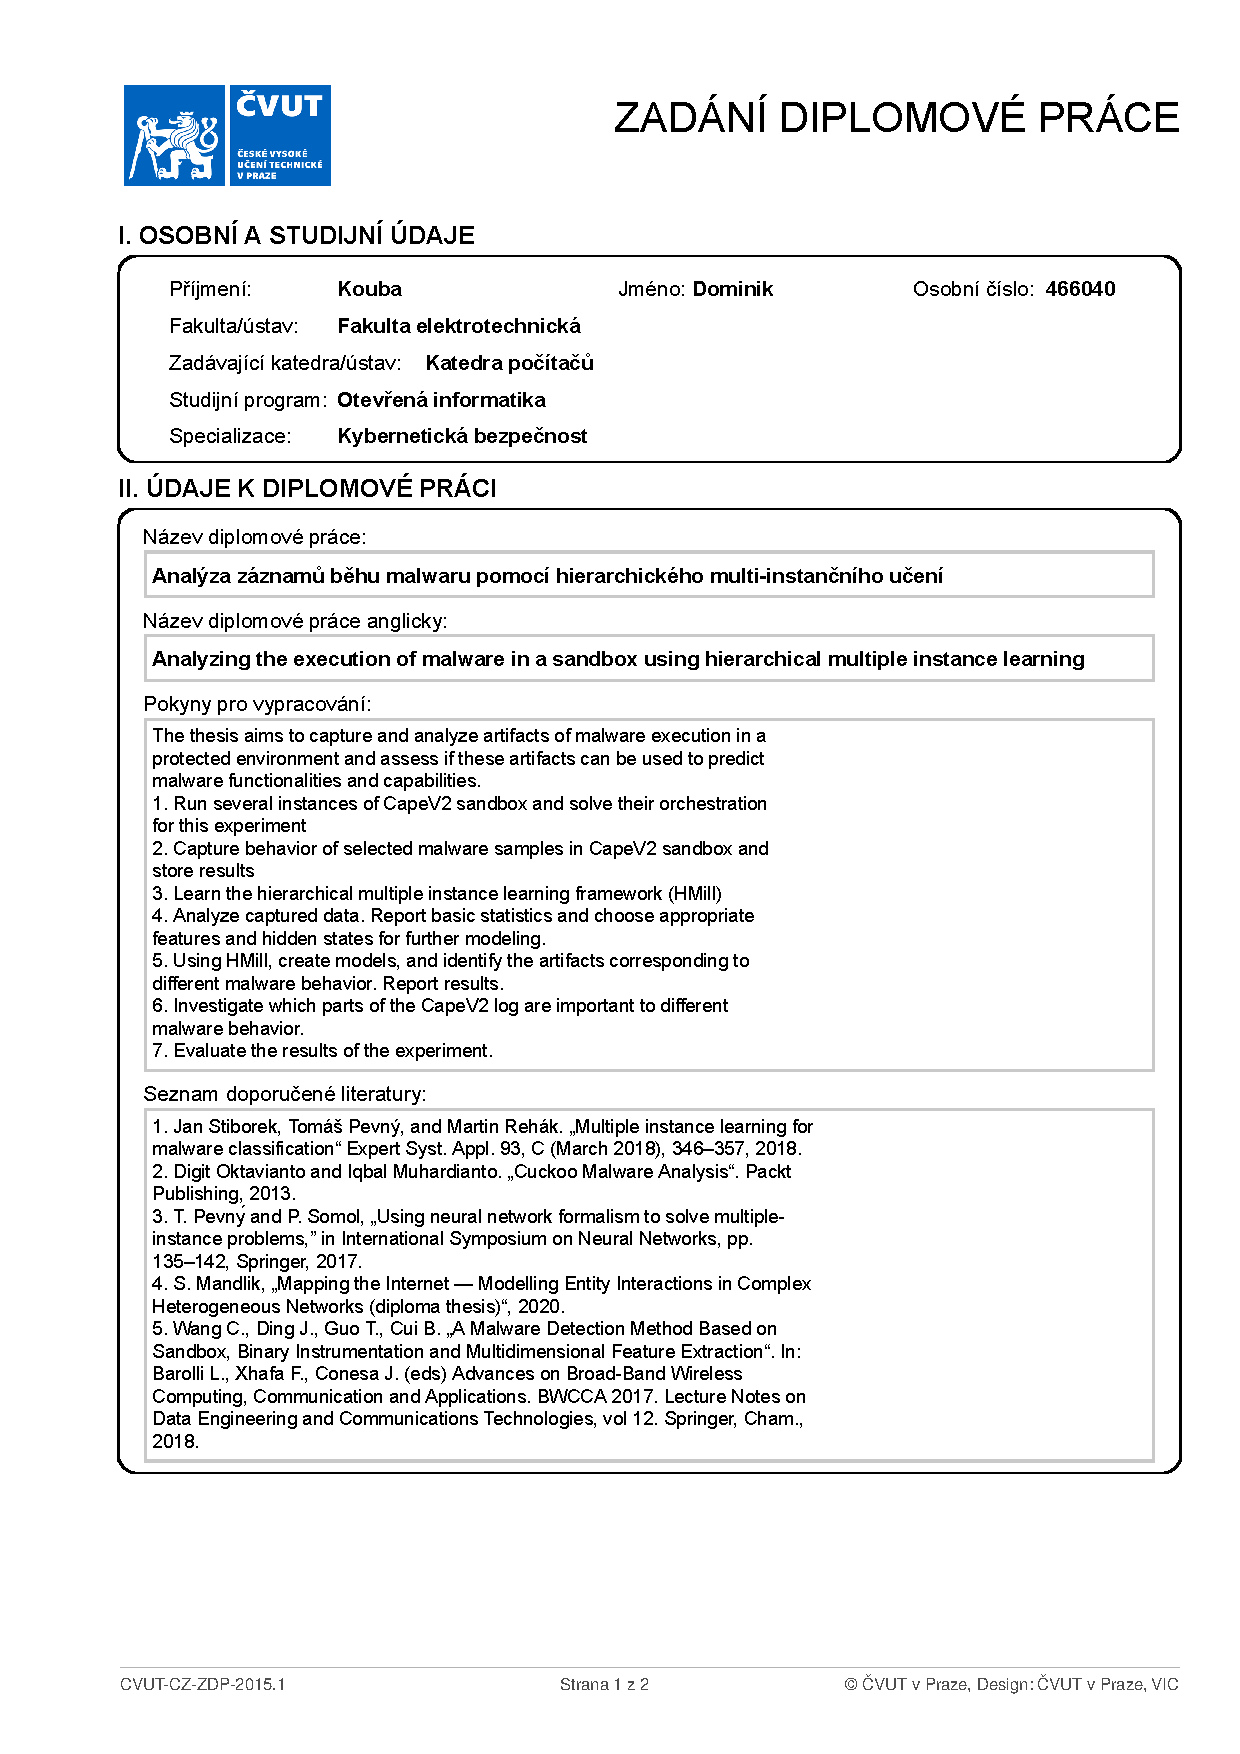
\includepdf[pages=-]{pdfs/zadani.pdf}
		\newpage
	}

	% Title page 
	\coverpagestarts

	% Acknowledgements 
	\acknowledgements
	\noindent
	My deepest gratitude goes to my supervisor doc.~Ing.~Tomáš Pevný,~Ph.D. for giving me advice and helping me overcome struggles during this journey. I also sincerely thank to doc.~Mgr.~Branislav Bošanský,~Ph.D., Ing.~Thorsten Sick and Ing. Josef Liška for their advice and encouragement. Finally, I wish to extend my special thanks to my family.

	\noindent\rule{\textwidth}{0.4pt}

	\noindent Computational resources were supplied by the project "e-Infrastruktura CZ" (e-INFRA LM2018140) provided within the program Projects of Large Research, Development and Innovations Infrastructures. This support was very beneficial.


	% Declaration 
	\declaration{In Prague on May 15, 2021}

 	%Abstract 
	\abstractpage
	In this thesis we focus process of malware classification based on behavioral analysis - sandboxing. We design pipeline which collect malware samples from defined sources, train classifier, evaluate and perform prediction explanation. The main goal is to implement whole process report results and address problems which we indentify. As malware sample source we used https://bazaar.abuse.ch/ and for its analysis we used sandbox CAPEv2. We use distributed setup of the sandbox run which we implement and the dataset has $80000$ samples. From the sandbox log we extract json report and its behavior part we use to train binary classifiers. As labels we use the presence of specific signature which are also in beahvior log. We use \emph{hierarchival multiple instance learning} model which is designed to solve even tree-structured data input (like JSON documents) as we can see from the prior work. The model itself is built based on input data structure and the underlying model are artificial neural nets. Based on the type of signature the classifiers have different performance but majority of them shows results above 95\% AUC. We discuss result in the case of each particular signature. Finally we examine the predictions of the classifier using \emph{hmill explaniner} which is tool designed to use statistical method to derive subsample from original sample which has the strongest contribution to resulting prediction of classifier. The results show us that explanation sometime correlate with the original signature implementation and even with our intuition. On the other hand we do not take the confounding variable existence lightly and we discuss results with sufficient distance. Main issue here is big data entrophy which causes big variance in explanations which are performed per sample. So each sample could be explained in very different way than another despite using the same classifier. \
	
	\vspace{5mm}

	\noindent Keywords: \emph{Multilple instance learning, cybersecurity, malware}

	\let\cleardoublepage\clearpage

	\noindent
	\chapter*{Abstrakt}
	\noindent
	In this thesis we focus process of malware classification based on behavioral analysis - sandboxing. We design pipeline which collect malware samples from defined sources, train classifier, evaluate and perform prediction explanation. The main goal is to implement whole process report results and address problems which we indentify. As malware sample source we used https://bazaar.abuse.ch/ and for its analysis we used sandbox CAPEv2. We use distributed setup of the sandbox run which we implement and the dataset has $80000$ samples. From the sandbox log we extract json report and its behavior part we use to train binary classifiers. As labels we use the presence of specific signature which are also in beahvior log. We use \emph{hierarchival multiple instance learning} model which is designed to solve even tree-structured data input (like JSON documents) as we can see from the prior work. The model itself is built based on input data structure and the underlying model are artificial neural nets. Based on the type of signature the classifiers have different performance but majority of them shows results above 95\% AUC. We discuss result in the case of each particular signature. Finally we examine the predictions of the classifier using \emph{hmill explaniner} which is tool designed to use statistical method to derive subsample from original sample which has the strongest contribution to resulting prediction of classifier. The results show us that explanation sometime correlate with the original signature implementation and even with our intuition. On the other hand we do not take the confounding variable existence lightly and we discuss results with sufficient distance. Main issue here is big data entrophy which causes big variance in explanations which are performed per sample. So each sample could be explained in very different way than another despite using the same classifier.

	\vspace{5mm}

	\noindent Keywords: \emph{Multiinstanční hierarchické učení, kyberbezpečnost, malware}

	%%%%%%%%%%%%%%%%%%%%%%%%%%    
	% obsahy a seznamy
	\tableofcontents		% Obsah / Table of Contents 

	% pokud v práci nejsou obrázky nebo tabulky - odstraňte jejich seznam
	\listoffigures			% Obsah / Table of Contents 
	\listoftables			% Seznam tabulek / List of Tables

	%%%%%%%%%%%%%%%%%%%%%%%%%% 
	% TEXT
	\mainbodystarts

	%Chapters
	\part{Theory and prior}
	\chapter{Introduction} \label{chap:intro}
\section*{Motivation}
Nowadays, we face an intense explosion of machine learning applications in various branches of human efforts. We can see applications in biology, chemistry, physics, and others. These technologies are influencing our daily life. They make it easier, faster and more enjoyable. On the other hand, we can see cases where algorithms (especially in machine learning) can control ourselves, our decisions, reasoning, and life.

If we use these computer science tools in a good way, we are often able to create something that may serve our protection. As an example, we can see the detection of threats and frauds in cybersecurity. Research and applications in this particular field are fascinating for multiple reasons, and one of them is motivation. We have to know which side we are standing on and what are the interests of our client.  In the case of fraud detection, we know that the investment is profitable only if the fraud has a significant financial impact. Not all frauds are interesting from the financial point of view because solving them also costs a lot of money. However, from an ethical point of view, every fraud should be punished. 

Similarly, network security, single device security and access control are considered to be applied later or never. Small businesses which are aiming at a specific market are not interested in some stuff which costs much money, and its main impact is preventive. The main role plays financial profit and costs reduction. Nevertheless, nobody wants privacy or data loss. It is often impossible to achieve both. We have to start with an analysis of costs, benefits, risks, their probability and impact (potential damage). This is not so evident in a technical branch as cybersecurity is.

The inseparable character of this play is malware. Let us motivate this thesis by listing several examples.

Firstly, one of the most prevalent malicious software is \emph{ransomware}. Its overall damage is estimated to be $\$20$ billion, and it increases every year \cite{purplesec2021}. The social impact is even more significant than the amount of money. We can see even attacks aiming at healthcare organizations. The first death reported following a ransomware attack was reported in 2020 \cite{Cimpanu2020}.

In Sonic Wall's 2019 report, we can find that IoT malware is becoming more common. It is caused by insufficient protection of these small devices, where we cannot provide complete malware protection. However, $127$ new IoT devices are connected to the internet every second. This leads us to estimate that by the end of 2021 we have 35 billion IoT devices connected to the internet \cite{TheIoTRu52:online}. This risk can not be mitigated easily, and malware elimination will play a significant role as it did so far.

Another convenient trend for malware is widespread encryption which becomes a standard in web traffic. Its main goal is the security of information. However, the creators of malware have much to hide and secure against the protectors, too. The encryption might inform us that the source has something that nobody else should see. A long-lasting trend of such behaviour might be suspicious. We can check if there is a justified reason, or we can at least make some conclusions. But not in a world where everything is encrypted.

$94$~\% of malware was delivered by email in 2020 \cite{Topcyber13:online}. The importance of phishing emails with malicious attachment and other social engineering techniques grows. It is cheaper to produce one sophisticated, convincing email to retrieve some information than attempt to attack a highly protected network perimeter. It also might be used to distribute malware or other threats.

In 2020 AV-atlas \cite{AVATLASM39:online} recorded over 750 million malware samples. At the end of April 2021, it was already 820 million malware samples. The majority of them are executable files attacking windows devices.

Malware research continues, and it undoubtedly will unless we can introduce a solution that is sufficiently universal and flexible to be able to detect zero-day threats (unseen). We might find a solution among machine learning models, which are often involved. However, its challenge is interpretability and explainability, not only in cybersecurity. We face the problem that the performance of the model is often significant, but we are not sure why. It is risky to deploy such a model to a situation where it can meet unseen data. High-quality security engineers do not have to be high-quality machine learning engineers. If we want to involve machine learning methods more and more, we need to be able to interpret and explain its predictions. Then we can combine knowledge from cybersecurity with the results of models and gain a better understanding. 


\section*{Goal}
The main objective of this thesis is to design a pipeline that has a malware file dataset as input and a machine learning model and its explanation as output. We want to go through the whole process, document each step and report results. Our acquisition is the process itself, it is described in detail for the reader to be able to identify problems we experienced and to be able to replicate or extend our setup.

From the assignment of this thesis, we can extract the following steps:
\begin{enumerate}
    \itemsep0em 
    \item Run several instances of CapeV2 \cite{Cape} sandbox and solve their orchestration for this experiment
    \item Capture behaviour of selected malware samples and store results
    \item Learn the hierarchical multiple instance learning framework
    \item Analyze captured data. Report basic statistics and choose appropriate features and hidden states for further modelling
    \item Using HMill, create models and identify the artefacts corresponding to different malware behaviour, report results
    \item Investigate which parts of the CapeV2 log are important to different malware behaviour
\end{enumerate}

The first step implies that we will use dynamic malware analysis to retrieve input for our machine learning model. This is motivated by a couple of thousands of sandbox \emph{JSON} reports we downloaded from the internet and examined. This dataset was not sufficient to observe significant performance. However, it was sufficient to realize that this use case is interesting for further research.

The initial task is data collection. We are about to use \url{https://bazaar.abuse.ch/} as a public data source of malware samples. We chose it because of its free access with no claims in usage and a reasonable amount of samples. We aim at \emph{Portable Executable} (PE), which does not require any additional software running on the target machine. The sandbox we want to use is \emph{CAPEv2} \cite{Cape} because first reports were also produced by this tool, and they are sufficient for analysis purposes.  It is a fork of popular \emph{Cuckoo} sandbox which is no longer maintained. We need to deal with distributed run of the sandbox to be able to collect a sufficient number of samples.

The model we want to use is \emph{hierarchical multiple instance learning} model. In \cite{Mandlik2020} authors showed that this model has significant performance modelling \emph{JSON} documents. We describe it and its alternatives in the first part of the thesis. 

After further research, we decided to model the dependence of malware \emph{signatures} on behavioural features, both presented in \emph{JSON} report. Signatures are the essential input for the original classification techniques used by the sandbox, and we want to see how well the model predicts them based on malware behaviour. We can study the implementation of signatures and their true cause, it might help us with results evaluation.

Finally, we will attempt to explain predictions by choosing a minimal subset of features that contributes to the model predictions the most. The explanation will be performed using the existing \emph{HMill} explainer. Its results will be compared to the original cause of signatures.

\section*{Thesis structure}
The thesis is divided into two main parts. In the first part, we focus on the theoretical background of our method. In the second part, we present a specific setup, our results and their discussion. At the beginning of each chapter is mentioned its particular goal. More complex structures (images, tables) are part of appendices. The thesis also has some attachments, including code, results and examples. These are described in \ref{app:attach}.

The theoretical part starts with the malware analysis theory in chapter \ref{chap:analysis} where we break down the malware itself, types of its analyses and its output. We continue in chapter \ref{chap:classification} where we describe machine learning formalism, cybersecurity context and structured data (\emph{JSON} document) usage in machine learning. Finally, chapters \ref{chap:hmill} and \ref{chap:expth} describe particular methods used in our modelling and explaining experiments.

The second part consists of two chapters. Chapter \ref{chap:infrastructure} includes description of used infrastructure and data collection process. Chapter \ref{chap:results} presents model and explainer setup, results and their discussion.




% The second part breaks down the use case we have. The first chapter \ref{chap:infrastructure} describes malware analysis sample collection, infrastructure and tools used to do that. Following two chapters contain description of the data and reasoning on how to use it and description of training process - hyperparameters, different models, conditions. Finally, last chapter is \ref{chap:expex} where we summarize the model explanation and its results. Crux of the thesis is the dicussion in the chapters \ref{chap:models} and \ref{chap:expex}where we address the model performance and explanation achievements and problems. We follow this discussion in the conlusion and in the formulation of goals of future work.


% The subject of this thesis is malware classification which is part of threat/intrusion detection. We want to use specific machine learning tool - \emph{hierarchical multiple instance learning} to train classifier on the data which we collect ourselves using dynamic malware analysis (\emph{sandboxing}). Our goal is to use data in \emph{JSON} format because this format is quite common output of reporting modules of sandboxes and usualy include majority of the information in structured form. The other reason is that the framework we are about to use shows significant results using such data.

% After we train the classifier (or several) we measure its performance and explain its predicitons. By explanation of predicition we mean using statistical method to extract the most important parts of input vector which contributed the most compared to other parts. Finally we discuss the performance of classifiers and the output of explanation.

% The model could be used to detect malicious code execution based on its behavior and later the explanation can be used to generalize some of our deterministic ways to detect malware (family assignment, signature marking) or just to explain what is for some specific malware family some generic group of malicious programs.

% There are experiments in each part of our task but we would like to examine the whole pipeline to see if we are able to go from plain malware sample to predictor which is explainable. We do not aspire to dig deep in some specific part rather we want to connect each step and identify problems which are in the whole process. We want to see it from a greater prespective. The whole process itself is acquisition and we want to demostrate all the steps.
% \todo{We can add some references}
% \section{Goals}




%%---------------------------------------------------------
% The structure of this thesis follows the steps which we defined in assignement but we solve theoretical point of view and our use case into two parts of this thesis.
% Text is organized such that each chapter focuses on specific goal from the assignement. Firstly we describe theory and prior work, further our conditions, experiments and conclusions.

% The main goal of this thesis which we are aiming at is to capture and analyze artifacts of dynamic malware analyses and draw conclusions in each part of the process. 

% - motivation
% - Motivation behind the modelling itself (classifying itself)
%   - classifying accordig to dynamic analyses, prior arts....
%   - My thesis is more practical, so the main goal is not to compare my results to another ones, but just demonstrate acuuracy of such classifier and everything around like for instance sandboxing, exaplaining
% - goals
% - structure of the thesis

	% \chapter{Malware analysis}
The data which we are performing analysis on are malware analysis results. Specifically those are dynamic analysis of running Portable executable (PE) files in sandbox environment. In this chapter we cover theory of malware analysis and everything related. \todo{add some motivation example or latest results... - known malware attacks..}

Philosophy could be walking around risk management, probability of risk and resulting damage... Maybe more examples of situations where we know how much it cost (Cambridge analytica, ransomware...)
Maybe something about truth and its protection in the world of lies and fake news
Confidentiality, integrity and availability

Use found books or post-hoc go through some articles and formulate the motivation part...


\section{Challenges}
Data quality, bias, antisandbox detection... where to find samples? (we should definitely mention motivation why we are collecting our own data), public data (this is quite risky to publish in general), everything is fast (zero days), Are those anomalies or malicious?, Imbalanced data sets, encryption everywhere - what to trust..., cryptocurrencies, iot, cloud

https://www.groundai.com/project/machine-learning-in-cyber-security-problems-challenges-and-data-sets/1
https://www.readitquik.com/articles/security-2/cybersecurity-challenges-that-need-to-be-on-your-radar-right-now/


\section{Malware}
Generally types of attacks and just the intro, to settle the malware into wider context
Definition of cleanware and malware
Types, Families
https://en.wikipedia.org/wiki/Malware
Find in books!

\section{Portable executable files}
Malware is defined widely and is not limited to specific kind of file format. In our research we decided to investigate only Portable Executable (PE) files. It is because we want to create dataset of malware running on windows machines with no extra extension. 

In general we can find various filetypes. In list below we list some examples with basic principle how particular type is used for system intrusion or harm. From the definition of malicious code we can derive that whichever filetype could by used but some are more usual than another (easier to use).
\begin{enumerate}
  \item Portable executable
  \item Portable Document Format
  \item Microsoft office formats
  \item Compressed
\end{enumerate}

https://en.wikipedia.org/wiki/Portable_Executable
https://docs.microsoft.com/en-us/windows/win32/debug/pe-format
https://github.com/corkami/pics/blob/master/binary/pe101/README.md

\section{Malware analysis}
introduction

https://en.wikipedia.org/wiki/Malware_analysis
Find in books!

\subsection{Dynamic}
https://publications.sba-research.org/publications/malware_survey.pdf
https://link.springer.com/article/10.1007/s11416-007-0074-9

mention especially parts which gives more information about the run (mutexes, files, api calls,.. - to be able to reference from data chapter)

- Summary of potential sorces of metadata
○ Abuse.ch - https://bazaar.abuse.ch/api/#api_key
○ VirusTotal - https://developers.virustotal.com/v3.0/reference#file-info
○ Metadefender - https://onlinehelp.opswat.com/mdcloud/3.1_Retrieving_scan_reports_using_a_data_hash.html
- Interesting
○ https://app.any.run/
○ https://virusscan.jotti.org/
○ https://virscan.org/
○ https://mzrst.com/
○ https://github.com/maliceio/malice
https://www.hybrid-analysis.com/

\subsection{Static}
○ Retdec - static analyser
§ Not so well documented..
§ I am studying the output, there is decompiled code and there some metada
§ I will use as it is out of box - decompiled code and some metadata
○ Manalyze
§ Another metadata like clamav signatures and something else


\section{Sandboxing}
existing solutions and results...
find basics in books


\section{Produced data}
mention signatures
usual format which are produced by sandbox and what we can find there
Reference even docs - no problem, not only books and papers
Conclusion should be that those data are complicated and their structure also keep some information (order, structure...), that is why we want to focus on structured data and especially json.


\section{Prior}
works about malware analysis
works that collected data for machine learning purposes
Mandlik, Stiborek, everybody who used cuckoo or other sandbox data

file:///C:/Users/domia/Downloads/Imad-Saiida-IJCNIS-V11-N6-1.pdf
https://web.archive.org/web/20160418151823/http://www.ijarcsse.com/docs/papers/Volume_3/4_April2013/V3I4-0371.pdf
https://reader.elsevier.com/reader/sd/pii/S1383762120301442?token=81F1AB06FF0FE40D1B7745234269280FCF2CB0979140E84DB35D6E04A2C622FE6EDA2DE4DA0630E1D73044E3D84A722F&originRegion=eu-west-1&originCreation=20210401090943
https://iopscience.iop.org/article/10.1088/1742-6596/1140/1/012042/pdf
file:///C:/Users/domia/Downloads/JCIT4024PPL.pdf
https://dl.acm.org/doi/abs/10.1145/2046614.2046618?casa_token=MXpfHiylCZcAAAAA:szRMPWfKXTl4wxP2-h32eknCg5dzM2t7RxGjywiJDksmT5FqcUY7pPrIBZchv26HUe3Lwubu5Hru




Previous connection
- Nothing before
Way through this chapter
- Malware definition and types
- Malware analysis
- Challenges
- Data - input, output...
- prior
Next connection
- We are interested in modeling the data using modern approaches, we know that the data are often structured somehow and that is what we will solve

- GOALS
  - Run several instances of CapeV2 sandbox and solve their orchestration for this experiment
  - Capture behavior of selected malware samples in CapeV2 sandbox and store results
- Theory part - types, conditions, bias, Malware types, signatures....
- Sandboxing
- Previous experiments
- Our goal in this part
- Data collection for ML purposes in general
	%\chapter{Malware classification}
We can expose a lot of information from malware analysis result. It contains api calls, network requests, downloaded payload and much more. This could be used to explain directly what is going on during the run. Sandbox itself is often labelling malware samples using so called signatures. These signatures are deterministically assigned amd usually sign that particular malware example is doing something suspicious (more later). Based on signatures we can later distinguish between different kinds of malware or between malware and cleanware - classify. Besides this deterministic way modern approaches from machine learning are often used.

This capture focus on classification problem in general and later in case of malware. We involved more theory and prior work research in following chapters we discuss our way.

\todo[inline]{
    Remainders:
    Malware analysis results could be used
    Following data collection and processing next task is  
    Based on type of analysis and characteristics of collected data
}

	% \chapter{Hierarchical Multiple Instance learning} \label{chap:hmill}
The goal of this thesis is to use specifically hierarchical multiple instance learning to classify malware samples. Using it we want to follow the prior work in this area \cite{Mandlik2020}.
In this chapter we describe multiple instance learning as extended approach compared to previus chapter. In the second part we will describe hierarchical multiple instance learning framework as modelling tool to model tree-structured data. Finally, we will address its usage in malware classification and other applications in cyber security field.

\section{Multiple instance learning - Mill}
At first let us describe and define problem of \emph{Multiple instance learning} its origin and formalism.

The most cited original article in this field is \citet{Dietterich1997}, it is not the very first formulation of such problem (it is in \cite{Keeler1991}) but fist usage of term \emph{Multiple instance learning}.

On figure \todo{reference figure} we can see basic idea behind \emph{Mill} problem. Standard learning described in chapter \todo{ref chapter} we can see as a special case of \emph{Mill}. Compared to defined formalism we have to change definition of \emph{example} \todo{ref section example in chapter 1}. 
\paragraph{Example}
Firstly we for our puprose we assume that we are in \emph{supervised} setting. Our examples consist of two parts - \emph{bag} $$b$$ and \emph{state} $$y$$. State was defined earlier and its meaning is the same but it is related to bag and sometimes called \emph{bag label}. \emph{Bag} $$b$$ is set of feature vectors $$x_i$$, these vectors are called \emph{instances} and usually lives in standard feature space $$x_i \in \mathbb{R}^{n}$$. Its length is $$|b| \in \mathbb{N}$$ and can be even zero. We assume that $$b \in \mathcal{B}$$ which denotes \emph{bag space}. \emph{Bag space} might also be seen as $$\mathcal{B} = \mathrm{Fin}(\mathcal{X})$$ which denotes all finite subsets of $$\mathcal{X}$$. Now we can see that standard learning is just \emph{Mill} problem where holds $$|b| = 1$$.

For the purposes of our thesis we assume mill classification problem so $$|\mathcal{Y}|$$ is finite. One more additional note is that some researches and even the original has one assumption (sometimes called \emph{Standard assumption}). This assumption is about underlying \emph{instance label} and their relation to \emph{bag labels}. This assumptions is often relaxed \cite{Xu2003} so even we do.

\todo{I have to mention some citations the theory I built on top of Mandlik and Amores!}

\todo{image of standard setting vs mill setting}

\todo{if we would like to have some fancy figure we can try something with keys}

The motivation example in original paper \cite{Dietterich1997} is formulated in following way. Imagine we have keys and some of them unlock specific door and some of them not (no other choice). Important is that we do not have access to the door. In standard learning is our goal to learn classification model which consumes key and outputs if it is able to open or not. But in \emph{multiple instance learning} setting we receive whole chains of several keys and without checking every single key we have to classify if the whole chain is able to open the door.

More on this topis we can find in \cite{Amores2013} where we can find formulated paradigms of solving such issues.

\todo{List paradigm and shortly describe and add some examples (prior) of solutions - cite}

\todo{some real world examples (not only pevny and Mandlik).}

\todo{Last solution describe neural net architecture - cite Somol, Pevny, Dedic (3 papers) and even Mandlik with the notation on page 14,15}
\todo{Mention Zaheer with deep sets}
\todo{Add own figure of neural net architecture}

- Prior experiments
    - Add something from another domain
    - https://www.etsmtl.ca/Unites-de-recherche/LIVIA/Recherche-et-innovation/Publications/Publications-2017/mil_marc_2017.pdf
    - The most impotant
        - https://link.springer.com/content/pdf/10.1007%2F978-3-319-59072-1.pdf (somol, pevny)
        - https://dl.acm.org/doi/pdf/10.1145/2996758.2996761
        - Stiborek - https://reader.elsevier.com/reader/sd/pii/S0957417417307170?token=492DD375F9C6F2836E0F6B394FAA2BC3E6663F3EFD26E24D7295DBFDCB870D23C3B120BCCC9731B0E6399BEFEE29C4A2

        - https://arxiv.org/pdf/2002.04059.pdf - Pevny, Dedic
        - https://arxiv.org/pdf/1906.00764.pdf - Pevny Kovarik, 
        - https://papers.nips.cc/paper/2017/file/f22e4747da1aa27e363d86d40ff442fe-Paper.pdf - same idea, but different name (just marginally)

\section{HMILL framework}
The idea of the neural net architecture by \todo{ref names Somol and Pevny} was followed by \todo{ref Mandlik and Pevny}. This led to formulation of \emph{HMill framework} in \cite{Mandlik2020} which refers to \emph{Hierarchical Multiple instance learning framework}. This framework builds on the top of the idea of hierarchically composed models. Inspite the fact that the hierarchical learning is generalization of standard learning we can cover quite complicated structured data (which is later used by us).

- Framework definition
    - go to Mandlik
- prior will be sufficient
    - Mandlik's results using the framework
    - https://arxiv.org/pdf/2002.04059.pdf

The conclusion of this chapter and maybe the most significant conslusion for our work is that it is possible to use \emph{HMill framework} to classify tree-structured data e.g. \ \emph{JSON} documents. \citeauthor{Mandlik2020} presents convincing results (for example on \emph{device identification} example) and that is why this framework is directly in assignment of this thesis.

Regardless of quite comprehensive theory which is covered in this part of the thesis, \emph{HMill} framework is still not everything. Our goal is quite cross-cutting and the model we are going to train we want also explain. What we mean by explanation we describe in next chapter.

%---------------------REMAINING-------------------------------------

HMILL:
- assumptions - https://en.wikipedia.org/wiki/Multiple_instance_learning (Be aware, I think those are not true all at once...), also algorithm list is presented, could be mentioned, and other interesting references like problem generalization
- between modern approaches mention adapting of single instance algorithms

Previous connection
- We focus on structured data and our tool is hmill, let's describe it
Way through this chapter
- multiple instance learning
- hierarchical mill
- prior
    - Prior in various fields
    - Prior in cybersec
Next connection
- Not necessary, but can connect to next chapter slightly (we want to explain this kind of model)

Stand on Madlik chapter, his citations (be aware), somol and Pevny


- GOALS 
- Learn the hierarchical multiple instance learning framework (HMill)
- describe theory, connect it to classical approach
- Usual usage of this type of learning - classification, regression...
- Our usecase and experiments with this kind of learning in malware classification field (prior)
	% \chapter{Model explaining}
In case of complex model structures like artificial neural nets we often want to explain its predictions. For example in case of malware we may be sure that the information used by the model is quite simple and straight-forward compared to the whole sample or at least that is in our expectation. That is why we often try to explain the models results to see if the explanation (e.g. \ subset of original sample which gives the model majority of information based on which it classifies) is hand in hand with our intuition. It could also be kind of hand brake to see that the model is not generalizing based on something relevant. For example in base prior article for us authors identified that their model is classifying mainly according to timestamp field in original sample, which was different for malware and for cleanware \cite{Pevny2020}. This was obviously mistake because this detail is not the difference between malware and cleanware.

Going from popular quote: \say{All models are wrong but some of them are useful} \todo{add name George E.P. Box} We should ask: \emph{What kind of model is useful?}
One of the greatest advice in machine learning and statistical data analysis is that less is more. If we are modeling some unknown process based on given data we should start from the simplest model and incrementaly proceed to more complex. This fact is derived from \emph{Bias x Variance tradeoff} \todo{Maybe some citation} and we can see practical consequences during model extrapolation but we can see even interpretability and explainability. That is why our next question should be: \emph{Why should we trust the model?} \cite{Ribeiro2016}.


\todo{another good motivation}
The European Parliament recently adopted the General Data Protection Regulation (GDPR),
which has become law in May 2018. An innovative aspect of the GDPR are the clauses on automated decision-making, including profiling, which for the first time introduce, to some extent, a right of explanation for all individuals to obtain “meaningful explanations of the logic involved”
when automated decision making takes place. Despite divergent opinions among legal scholars
regarding the real scope of these clauses [36, 74, 126], there is a general agreement on the need for
the implementation of such a principle is urgent and that it represents today a huge open scientific
challenge. Without an enabling technology capable of explaining the logic of black boxes, the right
to an explanation will remain a “dead letter.” \cite{Guidotti2018}

A lot of articles like \cite{Zhang2016} leads us to conclusion that neural net generalization is against our intuition or expectations. Let us introduce basic facts about model 
explanation and later about \emph{HMill} explaining.

This field is a little bit like a border between artificial inteligence, philosophy and other branches. We do not aspire to cover everything, the goal is to summarize terminology and basic challenges. This part of the thesis is more experimental, just to see what results we have and how we can interpret them.

\section{General approaches}

Notes:
Two main phases I think which are model explaing using some method and second is intepretation - human understandable
post-hoc intepretability X directly model interpretability
Explaining model X explaining particular predictions
local X global explanation
correlation X causality
definitions - basic terms (like for instance concept, math formalism...)

\cite{Montavon2018}
Techniques of intepretation and explaining are growing in popularity as a tool for further statistical model analysis. It might lead to better model understanding or it can shed some more light on examined domain (extract new knowledge) \cite{Montavon2018}

Deriving to \cite{Montavon2018} we can define two basic terms.
\begin{definition}
An \emph{iterpretation} is the mapping $$\mathcal{Y}\rightarrow\mathcal{D}$$. $$\mathcal{Y}$$ was defined in \todo{ref chapter Classification}) as \emph{state space}, in general it can be any kind of abstract concept (real-valued vectors, sequences\dots).  $$\mathcal{D}$$ denotes domain which is human-readable and understandable (image, heatmap, sequence of words\dots). Typically $$D$$ is the same as feature space \todo{define feature space} $$\mathcal{X}$$ or its transformation.
\end{definition}

\begin{definition}
    An \emph{explanation} $$e \in \mathcal{d}$$ is a subset $$e$$ of a interpretable domain $$\mathcal{D}$$ that contributed for the predicted state $$y \in \mathcal{Y}$$ (or contributed significantly more than other members and so it is cause of the result).
\end{definition}

This definition is quite vague because human-readability and understadability is not something to measure or observe precisely. We might assume that the original \emph{state space} is not straight-forward for human understanding which is usually true e.g. \ neural net's predicted class (just 1 or 0). In case of a neural net we can see only its parameters i.e. \emph{weights} and \emph{biases}, input features and than prediction. But the question is \emph{Why?}. Fortunately, final layer (or funciton) in neural network is \emph{softmaxx}, so we can try to interpret class probabilites instead just 1 or 0 outputs. We might want to see the subset of input features which is responsible for the majority of accumulated class probability. This subset should be intepretable by human as mentioned in definition because we are examining one blackbox and we do not need another. In our example we can assume images as input feature, so the explanation might be heatmap with highlighted significant pixels \cite{Lapuschkin2015, Simonyan2014, Landecker2013}. If the our subject would be natural language processing the explanation might by highlighted significant text \cite{Arras2017, Li2016}.

We often express explanations as original feature vector with some kind of relevance score vector e.g. \ real-valued vector of same dimension as input where positive items indicates relevant features and zeros irrelevant \cite{Montavon2018}.

Speaking about human readability and understand ability. Different point of view on 'measuring' it is to look at the available time which the user (human) is available or allowed to spend on understanding the explanation \cite{Guidotti2018}. Then we can check the complexity or quality of the explanation by measuring the time to understand the explanation and if its average is above required treshold. Of course this we can observe under the assumption we know (and can check) level of the background knowledge of person performing the interpretation. And this leads us to next complication \cite{Guidotti2018}.

Nice-to-have:
\cite{Mittelstadt2019}
section about Human explanations are selective - just to philozophy it a little bit



\cite{Lipton2016}
These definitions are not so rigorous how we would like them to be. We would rather state that another source of information is more clear but it is not. However, in \cite{Lipton2016} authors present very comprehensive, critical and real insight to desiderata of intepretability reasearch and an interpretable model properties.


\citet{Montavon2018} address the main bias in the term \emph{interpretability} and state that one of problems we face is that the majority of the model evaluation metrics works with the model as with blackbox - sufficient information for evaluation is just set of predicted labels (or class probabilities) and ground-truth labels \todo{maybe define those two}. Often, we do not observe model parameters, hyperparameters, model hypthesis space \dots. 

Another problem is that there are situations which are not easily trasferable to numerical form e.g. \ real-valued vector. Examples we can find in ethics or legality. Interpretability of such concepts is not ambigous even in the world without machine learning.


\todo{list Desiderata of Interpretability Research and summarize each and try to connect it to cyber security (examples, especially in case of huge data, huge entrophy and causality X Correlation tradeoff)}
\todo{make up some images, for example demostration of confounding variable}

\todo{add section about properties of interpretable model}

    We turn now to consider the techniques and model properties that are proposed either to enable or to comprise interpretations. These broadly fall into two categories. The first
    relates to transparency, i.e., how does the model work? The
    second consists of post-hoc explanations, i.e., what else
    can the model tell me? 

    \todo{summarize section properties of interpretable model, our model is post-hoc local I think so we can say something more about that}

    4.4. Post-hoc interpretations can potentially mislead
    We caution against blindly embracing post-hoc notions of
    interpretability, especially when optimized to placate subjective demands. In such cases, one might - deliberately or
    not - optimize an algorithm to present misleading but plausible explanations. As humans, we are known to engage in
    this behavior, as evidenced in hiring practices and college
    admissions. Several journalists and social scientists have
    demonstrated that acceptance decisions attributed to virtues
    like leadership or originality often disguise racial or gender
    discrimination (Mounk, 2014). In the rush to gain acceptance for machine learning and to emulate human intelligence, we should be careful not to reproduce pathological
    behavior at scale.

    we can also reference other authors in this field- \cite{Mittelstadt2019}
    Much recent work has been dedicated to rendering machine learning models interpretable or explainable. Two broad aims of work on
    interpretability have been recognised in the literature: transparency
    and post-hoc interpretation. Transparency addresses how a model
    functions internally, whereas post-hoc interpretations concern how
    the model behaves (Lepri et al., 2017; Lipton, 2016; Montavon et al.,
    2017).



If we know the model we are explaning and we can investigate its functioning, parameters and other details during learning process we speak about \emph{white box explaining}. On the other hand if we have only the output of the model without knowing what model is used and how it works we speak about \emph{black box explanaining}.

\cite{Guidotti2018} aims at blackbox models and their intepretability. Authors distinguish two points of view. - \emph{global} and \emph{local} intepretability of the model.

\emph{Global interpretability} means that we are able to intepret all predictions - we know intepretation $$f$$: $$\forall y \in \mathcal{Y}$$, $$\exists i \in \mathcal{D}$$ $$f: y\mapsto i$$. In another words the intepretation is mapping (or relation) and if the model is globaly interpretable this mapping is \emph{serial} (also called \emph{left-total}).

On the other hand \emph{local interpretability} means that we are able to intepret only some so mentioned relation is not \emph{serial}.


\cite{Guidotti2018} \todo{nice-to-have are another desiderata below}
Desiderata of an Interpretable Model
An interpretable model is required to provide an explanation. Thus, to realize an interpretable
model, it is necessary to take into account the following list of desiderata, which are mentioned
by a set of papers in the state of art [5, 28, 32, 45]:
• Interpretability: to which extent the model and/or its predictions are human understandable. The most addressed discussion is related to how the interpretability can be measured.
In Reference [32] a component for measuring the interpretability is the complexity of the
predictive model in terms of the model size. According to the literature, we refer to interpretability also with the name comprehensibility.
• Accuracy: to which extent the model accurately predicts unseen instances. The accuracy
of a model can be measured using evaluation measures like the accuracy score, the F1-
score [118], and so on. Producing an interpretable model maintaining competitive levels of
accuracy is the most common target among the papers in the literature.
• Fidelity: to which extent the model is able to accurately imitate a black-box predictor. The
fidelity captures how much is good an interpretable model in the mimic of the behavior of
a black-box. Similarly to the accuracy, the fidelity is measured in terms of accuracy score,
F1-score, and so on, but with respect to the outcome of the black box.

\cite{Guidotti2018} \todo{check consistency of my definition and theirs, maybe extend my to match and cite}
Definition 4.1 (Model Explanation Problem). Given a black box predictor b and a set of instances
X, the model explanation problem consists in finding an explanation E ∈ E, belonging to a humaninterpretable domain E, through an interpretable global predictor cд = f (b,X) derived from the
black box b and the instances X using some process f (·, ·). An explanation E ∈ E is obtained
through cд, if E = εд (cд,X) for some explanation logic εд (·, ·), which reasons over cд and X.


\citet{Guidotti2018} further categorize explanation techniques into several groups based on the basic princeple:
\todo{summarize the categories below, and we should also reference it in hmill explaining section also, what we use}
We further categorize in the subsections the various methods with respect to the type of interpretable explanator:
• Decision Tree (DT) or Single Tree. It is commonly recognized that decision tree is one of
the more interpretable and easily understandable models, primarily for global, but also for
local, explanations. Indeed, a very widespread technique for opening the black box is the
so-called “single-tree approximation.”
• Decion Rules (DR) or Rule Based Explanator. Decision rules are among the more human understandable techniques. There exist various types of rules (illustrated in Section 3.3). They
are used to explain the model, the outcome and also for the transparent design. We remark
the existence of techniques for transforming a tree into a set of rules.
• Features Importance (FI). A very simple but effective solution acting as either global or local
explanation consists in returning as explanation the weight and magnitude of the features
used by the black box. Generally the feature importance is provided by using the values of
the coefficients of linear models used as interpretable models.
• Saliency Mask (SM). An efficient way of pointing out what causes a certain outcome, especially when images or texts are treated, consists in using “masks” visually highlighting the
determining aspects of the record analyzed. They are generally used to explain deep neural
networks and can be viewed as a visual representation of FI.
• Sensitivity Analysis (SA). It consists of evaluating the uncertainty in the outcome of a black
box with respect to different sources of uncertainty in its inputs. It is generally used to
develop visual tools for model inspection.
• Partial Dependence Plot (PDP). These plots help in visualizing and understanding the relationship between the outcome of a black box and the input in a reduced feature space.
• Prototype Selection (PS). This explanator consists in returning, together with the outcome,
an example very similar to the classified record, to make clear which criteria the prediction
was returned. A prototype is an object that is representative of a set of similar instances and
is part of the observed points, or it is an artifact summarizing a subset of them with similar
characteristics.
• Activation Maximization (AM). The inspection of neural networks and deep neural network
can be carried out also by observing which are the fundamental neurons activated with respect to particular input records, i.e., to look for input patterns that maximize the activation
of a certain neuron in a certain layer. AM can be viewed also as the generation of an input
image that maximizes the output activation (also called adversarial generation).



prior
- each of papers presents their own approach wich could be mentioned
NN
    Motivation example - https://arxiv.org/pdf/1311.2901.pdf (quite often seen results )
https://arxiv.org/pdf/1806.07538.pdf
https://arxiv.org/pdf/1602.04938.pdf
https://link.springer.com/content/pdf/10.1007/s10115-013-0679-x.pdf
https://ieeexplore.ieee.org/stamp/stamp.jsp?tp=&arnumber=4407709
https://reader.elsevier.com/reader/sd/pii/S1051200417302385?token=E746E7B6AEA70FD3F88C8EDB1CE81407F166E7078D3011812BBC4D2DEB1597D112CCA6A919B515991126E136897B721C&originRegion=eu-west-1&originCreation=20210405200556 \cite{Lipton2016}



\section{Explaining HMill models}

\todo{could be good to formulate pseudocode of the explainer also}

Our target is explanation of \emph{HMill} model because it is also model we are about to use. In this section we will introduce solution proposed in \cite{Pevny2020} and we will reference other solutions which were presented on models capable consuming \emph{JSON} documents.

If we do not specify we assume binary classification setup.

As mentioned earlier we assume two main models capable processing tree-structured data. Those are \emph{Graph Neural Nets} and \emph{HMill}. Both methods described below are based on indentifying subset of original feature vector set (graph, tree-structured document) which has crucial role during prediction itself (in our case classification). \todo{connect to the theory above}

\todo{First shortly about gnn explainer and their results - https://cs.stanford.edu/people/jure/pubs/gnnexplainer-neurips19.pdf, https://arxiv.org/pdf/2001.06216.pdf - adaptation of LIME in graph neural networks (which also can solve our problem theoretically)}

\todo{Summarize MillExplainer - file:///C:/Users/domia/Downloads/Explainability_ICML2021.pdf}
Two main steps
    sub-trees in a sample are heuristically ranked to reflect their importance for the final classification
    subtrees of a sample are searched throughand evaluated by the model in order to find the minimalexplanation
Summarize mentioned ways
Summarize conclusions and results
    Conclusion The best way are Banzhaf values

Here or at the beginning of the section we should classify proposed solutions in context of the theory above. - our model is post-hoc local and quite complex in terms the data dimension..., also connect it to mentioned categories

\todo{idea: some kind of explanation is even more complex class hierarchy, I did not see the purpose in classifying something else than malware X cleanware, but the class hierarchy can give us some kind of clues}

\section{First part summary}
\todo{the section heading does not have to be presented}
Summarize main point in this part and motivate next part


%%------------------------------------------------------------------------------------


Previous connection
- Hmill models and their explanation
Way through this chapter
- Explaining in general
- Explaining mill and hmill
- Prior
Next connection
- Next should be little summary of first part of thesis


	\part{Usecase and experiments}
	% \chapter{Infrastucture and data collection} \label{chap:infrastructure}
This chapter describes the realization of the data collection process using \emph{CAPEv2} sandbox. The sandbox is described in the chapter \ref{chap:analysis}, here we focus on the specific setup, problems we experienced and their solution. In the beginning, we have a data source of malware samples mentioned in the thesis introduction https://bazaar.abuse.ch/. The output of this task is a dataset of dynamic malware analyses. It includes behavioural features and signatures, both input for our \emph{HMill} model.

Although this chapter is shorter than the previous ones, we spent the most significant time on this task. All scripts and other outcomes are part of the attachment (\ref{app:attach}), and the most important tools are listed in \ref{app:technologies}.

\section{Host machine}
The host machine is where the sandbox environment and virtualization software is running. We know that an analysis of one malware sample takes up to five minutes, and we want to have as many samples as possible. That is why we want to run several distributed host machines. 

The whole process of a host machine initialization is automated to be able to set up multiple machines. The initialization consists of several steps:
\begin{itemize}
    \itemsep0em 
    \item Install host operating system - recommended Ubuntu
    \item Enable SSH to be able to access remotely
    \item Enable basic security - firewall and supporting tools
    \item Install virtualization software - recommended KVM QEMU
    \item Copy virtual machine images to the host machine
    \item Sandbox initialization and configuration
    \item Data collection script initialization
\end{itemize}

To run all steps on multiple machines at once, we used Ansible, a network orchestration tool. We also added some usual management functions - copy new configuration from the server and clean up the sandbox data.

Hardware resources on host machines are 256GB SSD and 16GB RAM, which means that a sufficient number of virtual machines per one host is four. We experimented with more, but there was an overload which might lead to biased analysis results.

Various issues accompanied the automation of the whole process. Such a process often needs manual steps, and their automation was very challenging. Issues were caused mainly by our low experience. Sometimes poor documentation was involved. Especially the process of the virtual machine images creation and copying was connected with issues. Overall, we have configured seven host machines.

\section{Guest - virtual machines}
Guest denotes the machine where the malware sample runs and where the \emph{CAPEv2} monitor is operating. We used Windows 7 as an operating system. The crucial goal of the guest machine is to look like an ordinary computer that is in regular use. Due to virtualization usage, we have to care about sandbox evasion techniques mentioned in \ref{chap:analysis}.

There are two options for anti-evasion setup in \emph{CAPEv2} sandbox. Firstly, we experimented with vmcloak\footnote{https://github.com/hatching/vmcloak}. We were able to run and use this tool. However, it supports only VirtualBox, which is not recommended by \emph{CAPEv2} because of its performance. The project is also no longer maintained, and some functions did not work (taking snapshots). The second option is to use a script recommended by sandbox contributors\footnote{https://github.com/doomedraven/Tools/blob/master/Virtualization/kvm-qemu.sh} and perform manual steps in the virtual machine configuration\footnote{https://www.doomedraven.com/2016/05/kvm.html\#modifying-kvm-qemu-kvm-settings-for-malware-analysis}. After several unsuccessful attempts with misconfigurations in the low-level virtual machine configuration, we were able to create four working images.

The sandbox requires disabling of firewall and running python on the guest machine. We added the most popular applications like Google Chrome, Firefox, Adobe reader, Spotify\dots. We added one private key to C://Users/Administrator/.ssh and one password to the google chrome password database. We downloaded random images and documents from the internet.

\section{Network setup}
The network setup is a crucial point in the dynamic analysis. The guest machine has to reach the host machine to stay in touch with the result server. Secondly, there is an internet connection for the guest, which might be necessary for some malware types. As an example, we can see \emph{dropper}, which is responsible for downloading a payload.

We decided to collect the data under two different conditions - with internet connection (denoted by \emph{internet}) and without (denoted by \emph{none}). We engaged both because the \emph{internet} is much more difficult to set up and secure, and we wanted to start data collection as soon as possible. Both architectures are figured in the appendix \ref{app:network}.

\emph{None} setup is a straightforward option for an isolated network between host and guest. This approach requires a host-only interface created in \emph{KVM} virtualization tool. Host and guest are assigned with IP addresses from the same range. From a security point of view, we have to set up a firewall of the host machine. It should accept connections from the isolated network only on the result server's port.

\subsection{Internet}
We want to provide internet access to the guest machine during the analysis run. For this purpose, we prepared a VPN connection to the secured network through which all the communication should be forwarded. That is considered a good practice to observe what the samples are doing and be able to stop it fastly. This network we call \emph{dirty lab}.

\emph{CAPEv2} supports VPN connection setup for each guest machine separately. We knew that it would be better to have a central gateway for all local traffic than connecting each particular guest machines to \emph{dirty lab}. However, we decided to use native sandbox functions at first. After experiencing some issues with \emph{CAPEv2} VPN configuration and an unsuccessful issue-reporting, we decided to find another custom way. 

The main requirement is to centralize all the traffic from the local network (malicious) to \emph{dirty lab}. The exit point we call \emph{router}. The surrounding university network has to be secured and isolated from malicious traffic. We also need to monitor host machines because of external intrusion and centralize logs from host machines.

In the following text we use \emph{l2} and \emph{l3} as a designation referring to ISO/OSI model of network communication \cite{Zimmermann1980}. By \emph{l2} we mean communication on the data link layer. Specifically, we mean ethernet/802.11 local networks where MAC (Media access address) is used for device identification. By \emph{l3} we mean IP communication on the network layer. IP addresses are used for device identification in \emph{l3}.

An expert recommended the designed network architecture after a consultation. Its basic idea is to avoid \emph{l3} communication on the local network such that IP address from one range is assigned only to the guest machine and then to the router device. This idea was supported mainly by the \emph{l2} VPN on the local network.

The role of the router is to receive the traffic going out of the local network and forward it to the \emph{dirty lab}. It can also monitor and capture the traffic. In \emph{dirty lab}, we were provided with the ipv4 interface only, so the \emph{router} performs network address translation (NAT). \emph{Router} machine is running Ubuntu operating system. It is configured to connect to \emph{dirty lab} using \emph{l3} VPN and to the guest machines using \emph{l2} VPN. In \emph{l2} VPN, \emph{router} is a server and in \emph{l3} VPN, it is a client (server is running in \emph{dirty lab}). \emph{Router} is a virtual machine for fast recovery ability. All logs from the server are sent to the central machine.

The host machine has to be configured as a client in communication with \emph{router} using \emph{l2} VPN to forward the guest's traffic. The idea of this setup is that all the traffic leaving this device is encapsulated in packets with university network IP addresses. This network is unknown to the guest device where malware is running. From the guest's point of view, the connection between the \emph{router} and \emph{guest} is on \emph{l2}. 

On the host, the interface for \emph{l2} VPN communication (TAP) is bridged with the original interface, which allows communication with the guest virtual machine (originally host-only). 

A connection to the internet from the guest machine goes through the host machine, the router, the dirty lab, and the internet. 

There has to be performed additional setup on host machine besides these listed in case of \emph{none}. Each host machine in distributed cluster has to send all sandbox logs to the central Syslog server. All machines have to be set up with a monitoring tool to detect intrusion\footnote{example https://aide.github.io/}.

\section{Data collection pipeline}
During the distributed data collection, we used the following terminology. \emph{Master} is a machine responsible for sample distribution, and it has access to the NAS, where it stores analysis results. \emph{Worker} is another name for \emph{host} machine in the context of distribution.

This section describes the whole process of data collection from a malware sample over its dynamic analysis and ending with behavioural features and signatures extracted from the \emph{JSON} report. All programs implemented to solve mentioned problems are part of the attachment (\ref{app:attach}). Particular steps are automated, and their description follows.

\begin{enumerate}
    \itemsep0em 
    \item Download samples from the \emph{malwareBazaar}
    \item Filter PE files only
    \item Retrieve additional metadata
    \item Add hashes to database
    \item Distribute samples to workers
    \item Analyze sample and send result back
    \item Store result
    \item Extract JSON report
    \item Prune unnecessary parts
\end{enumerate}


\subsection{Abuse.ch malwareBazaar}
The place where we downloaded malware samples was abuse.ch\footnote{https://abuse.ch/} specifically its part called \emph{malwarebazaar}. The reason for its usage is its free access without any claims. \emph{MalwareBazaar} is a database of malicious (no benign files or Adware) samples where everybody can share and download. In May of 2021, it contains over 325~000 samples. Malware samples are downloaded in compressed form - one archive for every day since the start of the project.

\subsection{File filtering}
Our project aims only at PE files described in \ref{chap:analysis}. After decompression of original archives, we filter files based on the file extension and file headers. We also filter compressed files, decompress them and again filter PE files only.

\subsection{Metadata}
The secondary intention was to obtain some basic metadata about each file to have basic information about each sample. We were able to gain academic access to the VirusTotal API\footnote{https://developers.virustotal.com/v3.0/reference}. We downloaded a metadata report for each of our samples. The report contains basic static information like hashes and fuzzy hashes, extracted strings, detections of various antiviruses and even a summary of reports of used sandboxes.

\subsection{Distributed sandbox}
After dealing with issues in the host initialization part and even in the VPN setup part, we also encountered issues while setting up the distributed sandbox. \emph{CAPEv2} can orchestrate multiple host machines. It uses distributed mongo database\footnote{https://www.mongodb.com/} combined with a script that is run on the master machine to check the connection to registered worker devices. We spent with the configuration of distributed \emph{CAPEv2} large amount of time trying multiple different ways and following several pieces of advice but unsuccessfully. We decided to implement our lightweight solution for time reasons.

Hashes of our files are stored in a database (in our case \emph{JSON} file) with additional attributes. A script runs on the master machine that distributes samples among worker machines using their REST API. After the analysis is done, another script on the worker machine compresses the result and sends it back to the master. The last script manages coming results and saves them to the NAS. Everything is recorded in the database.

\subsection{Results postprocessing}
We need only part of \emph{JSON} log, specifically behavioural features and signatures, for further modelling. Its extraction was done in two steps. Firstly, we decompressed the analysis result and extracted only \emph{JSON} log. Secondly, we extracted mentioned parts and saved the shrank output. The whole report might have even gigabytes. However, the shrank variant has usually tens of megabytes. We could transfer the output to the metacentre where the model computation and explanation took place.

\section{Dataset}
When we start modelling experiments, we have a dataset consisting of $80000$ different samples in \emph{none} network setup. The \emph{internet} configuration took us several weeks to deal with, and the data collection started later and was slower. The \emph{internet} data will be investigated in future work as its collection continues. 

The complete dataset has approximately $2,5$~\emph{TB} in compressed form. Extracted features and signatures are much smaller (tens of gigabytes). 

Not all sandbox outputs described in \ref{chap:analysis} are presented in each analysis result. The configuration and other conditions determine it.

After examining the histogram of seen signatures, we chose a subset based on their frequency in the training set. We prefered signatures that are implemented in Python for convenient investigation of the original cause. In the \ref{app:signatures}, we can see our candidates, their frequencies in the dataset and additional information, including even the groups described in chapter \ref{chap:classification}.

% The data in such domain are very biased. Sometimes we can see that malware can not be run under the conditions in a guest or is trying to use some \emph{.NET} library and if not found, it kills itself. The fact that we do not have an internet connection can make this bias stronger, so we have to count on it to decide what to use to train the model. We do not want to investigate network activities even if sometimes it contains something (malware attempts).



% We have some of the results which were mentioned in \ref{chap:infrastructure}. When we start the following reasoning, we have the proper amount of the data without internet access because the setup is straightforward and more accessible. 

% \section{Results of analysis}
% The outputs of the previous chapter are dynamic malware analysed samples. Even such experiments used machine learning algorithms on all the produced data, but this is very performance demanding because the output may have 15~\emph{MB} but even gigabytes. That is why we want to choose the only subset containing the most information about the run and behaviour. 

% The goal of this thesis is to use \emph{hmill} model (comprehensively described in \ref{chap:hmill}), which can work with graph-structured data and especially with JSON files. This fact we would like to use.

% Our approach is to create a simple binary classifier and then scale up to multiclass or even multilabel if possible regarding performance and time. This chapter describes our reasoning on choosing features and hidden states for our \emph{hmill} classifier.  Collected results are input, and the expected output is a set of features and states (maybe more than one possibility). This decision should be based on the data we have and the experience observed in prior work.

% Complete description of the output of the sandbox is in appendix \todo{reference}.
% Description what everything we have at the end for every single sample, size of dataset (GB and number of samples)...
% Try to compare to another public dataset with the attributes and mention that using this way is quite universal
% What we have X what the docs says (caused our misconfiguration...) - https://cuckoo.readthedocs.io/en/latest/usage/results/ (reference cuckoo book)

% \chapter{Data structure, features and states} \label{chap:data}

% \subsection{Sample distribution}
% Reference scripts and crons..., sample storage
% problems using provided distribution (concretize some, extract from notes, poor docs,..)
% using nas storage and so on...


% First phase of our work is about running chosen sandbox to capture sigificant number of analysis results for further use. This task could be divided into two subtask - building infrastructure and data collection. Due to the fact that we would like to collect more than $50 000$ samples and usual analysis take $5$ minutes we will need more than one active instance so the distribution is another challenge.


% Download samples from abuse
% Filter samples by file type (PE) - filtered directly pe files and then extracted zip files and filtered again
% Add filtered samples to database (store in json file, which I backup regularly, later could be improved)
% Retrieve additional metadata for files (VT)
% Distribute samples to slaves (each file should be analysed in each mode, for distribution REST API of cape sandbox is used)
% Collect and store results

% VT, Metadefender and abuse reports, mention academic access for VT so we end up with that only

% There is some useful info in this data. But nothing totally awesome. But good enough for pre-sorting.
% Interesting are:

% Abuse.CH:
% - First seen: Us the oldest date to estimate how old the sample is. We need that for time scales
% - ssdeep: Fuzzy hash, good to find similar samples
% - sha256: Most common hash to link them together
% - md5/.../other hashes: Sometimes used in articles. Keep them for reference

% Metadefender:
% Multi-scanner. Be aware to check which Av detected it. Only use the top 10 (check out av-comparatives or av-test)
% Creation date is important. If the sample is older the AVs had some time to add detection (older: Time between first seen and detection)


% Virustotal:
% Similar to metadefender. Plus: It has update time of engine.
% The other data in here:
% - Packers: Malware can be packed. A nice hint, if available
% - Import list: Used DLL functions. Some malware is loading external functionality during runtime....
% - Resources: Attached malware parts (encrypted => high entropy). Maybe also abusing Icons of well known tools (=> trojans)
% - Signature: Could be helpful to weed cleanstuff our. If it is properly signed by a authority we can trust....
% If we want to classify malware as the first AV vendor seeing it, we can not use the detections others have on it. Obviously.
% HTH
% Thorsten

% figure of the setup, description, argumentation
% similar projects (isolation of malware network having internet access)
% two branches - no internet, internet
% internet
%     describe in detail
%     firewall
%     security resoning
%     syslog...
% safe network made our work easier, mention couple of further ideas mentioned by Josef (thank to Josef at the beginning of thesis!)


% add literally every detail including some scripts to appendix, even configuration of network, vpn, reference manuals, security reasoning during setting up internet connection (see notes)...

% Previous connection
% - Follow up analysis chapter and summarize what we did
% Next connection
% - At the end should be described output of sandbox and at the beggining of next chapter should be stated what we have chosen and why



% Possible sources
% Chosen source
% - recommendation from team member
% - description of Abuse.ch
% - possible problems - bias?, Emotet results?, Some statistic from the report from VT which I downloaded (nice-to-have), maybe could be quite interesting to retrive list of file extentions - histogram?


% 


% - Realization of chapter 'data'
% - our infrastructure - distribution, other types of analyses, network infrastructure (marginally, I am not going to use those data, I think, but I performed it and I can write about the risks and so on...)
% - used tools
% - distrbution
% - pipeline
% - run
% - results
% - Conclusions, comming-outs, summary, discussion


% \todo{absorb chapter about data here, describe the output and marginally discussion on what should be feature vector and classes (but present it as ready decision - from the introduction)}

% \todo{this chapter could be absorbed into next chapter if it is too short...}
% \todo{do not forget to add goals to each chapter and go through the trash below each chapter!!}


% Lastly thrown out
% We would like to base our decision on the fact that in \ref{chap:analysis} we stated that crucial observations during the program run are \emph{processes, files, mutexes, registries, commands, api calls}.

% \todo{avoid background things, that should be moved to analysis part, here strictly what we solved and architecture and so on}

% NICE to have
% We can try to create some histogram using the data from virus total (families or something like that...)
% \todo{checkout some web interface example, if there is something else, and even configuration files}
% \todo{add sections of report from virus total and its features}
% https://developers.virustotal.com/v3.0/reference#files
% \todo{add some image}

%%----------------------------------------------------------------------------------------------

% This statement is truth even physically such big data amounts we have to solve on bigger cluster like cesnet.metacenter. \todo{mention data amount before and after processing pipeline}
% After we decided which data parts are useful we used linux tools and Julia language to \todo{reference Julia in appendix technology description and maybe even lazyjson library} extract what we need from original analysis results \todo{reference what we used in bash - if necessary (maybe I can add to attachment bash script with trasformation like that if needed), and reference pruner code in attachements, we should have appendix description of attachments}


% "behavior
%     "processes, "processtree  - list of processes related to malware run with details (api name, arguments...)
%     "summary
%         "files
%         "read_files
%         "write_files
%         "delete_files
%         "keys
%         "read_keys
%         "resolved_apis    
%     "enhanced - detail sequence of events (library loading, api calls with parameters...)


% \todo{more about them we say in chapter on modelling, or maybe here give example of code and signature detection and data part (and all parts) and to appendix we can add more, with reference to the repository}

% Describe parts of json report
% JSON report parts \todo{describe that json report is quite comprehensive and contain even earlier mentioned outputs} \todo{to appendix we should add some example of report.json}
% - size vary a lot, could be from 10MB to GBs
% lack of docs - https://github.com/cuckoosandbox/cuckoo/issues/2458

% "statistics - time statistics for particular part of malware analysis
% "info - sandbox details (machine, category, used modul...)
%     "version"
%     "started"
%     "ended"
%     "duration"
%     "id"
%     "category"
%     "custom"
%     "machine
%     "package"
%     "timeout"
% "CAPE - extraxted payload
% "behavior
%     "processes
%     "processtree
%     "summary
%     "enhanced
% "debug - debug log of sandbox
% "deduplicated_shots - screenshots
% "network
%     "domains
%     "tcp
%     "udp
%     "dns
%     "pcap_sha256"
%     "sorted_pcap_sha256"
% "static - static analysis of files
% "strings - extracted strings (static analysis technique)
% "suricata - network detection Suricata tool log
% "target - sample details
% "malfamily_tag"
% "signatures - list of signatures and their data
% "malscore"
% "ttps

% paragraph about each and resoning on if we can use it or not, and what kind of analysis can be based on particular part (I think we enumerated almost all parts of original log)


% Summary of the data set - How many samples, size...
% Also we can try to specify the requirements for our model (quite big amount of data - all the reports), we are not able to process whole outputs, reference hmill capacities on previous experiments (for example in Julia language)


% \todo{Final result of data collection - no internet samples (maybe mention at the end of previous chapter), I did collect some, but did not use them in further parts because priority was not to have everything}

% Their analysis is in future work same as data from static analysis (Virus total). These data are still part of our data set and was big part of our job so far. So the subject of our research is sandox output.

% Previous connection
% - Follow up statements about data in cybersecurity, follow previous chapter with choosing relevant parts of logs
% Way through this chapter, we do not use internet access data, because we did not have it at right time, no internet data are sufficient for our further experimentation
% Next connection
% - Chosen data will be used for further experiments


% reference some source that is talking about data in cyber security, resp. on theory part

% Data processing
% extracting desired parts
% Is there something else in processing?
% Pruning jsons in Julia...

% reference that we did use similar parts as predecessors (Pevny, Mandlik, Stiborek)

% Detail descriptions of candidates, for example describe signatures (just describe what they do and sort them to categories according to what they are doing) and give example and at once slightly say why the signatures could be interesting (based on behavior like this we can validate model, such that it is using the proper part of report, but we can see whatever else which looks like malicious)


% Next chapter - Due to the data quality we are not able to use some of them

% Get several reasonings for some parts of analysis, what we want and we do not, also we can compare it to Stiborek and other works (for example Mandlik had quite straight-forward dataset and we know that it worked), we can really investigate the whole output and present ideas. 


% At the end we can have more variants, but at the end we did examine two and that should not be a problem
	% \chapter{Data structure, features and hidden states}
So far we know that sandbox output can is quite rich. There even such experiments that used machine learning algorithms on all the produced data but we would like to use some subset. In this chapter we describe our reasoning on choosing feature vector and hidden states.

Final result of data collection - no internet samples (maybe mention at the end of prevous chapter), I did collect some, but did not use them in further parts because priority was not to have everything

Technology - Julia
  - describe why and basic features and advantages and cons


How many samples, size...
Summarize what we know from previous sections and go to the most concetrated information about run of program - we should end at the things which are in summary part of json log, but we can have more variants
we can even mention virustotal reports here

Get several reasonings for some parts of analysis, what we want and we do not, also we can compare it to Stiborek and other works (for example Mandlik had quite straight-forward dataset and we know that it worked), we can really investigate the whole output and present ideas. Also we can try to specify the requirements for our model (quite big amount of data and we have to demonstrate on device we have)


Detail descriptions of candidates, for example describe signatures and give example and at once slightly say why the signatures could be interesting (based on behavior like this we can validate model, such that it is using the proper part of report, but we can see whatever else which looks like malicious)

At the end we can have more variants, but at the end we did examine two and that should not be a problem

Data processing
extracting desired parts
Is there something else in processing?
Pruning jsons in Julia...

Basic statistics for various parts and variants
  - signature histogram (balanced )
  - ...
  - a lot of Emotet (maybe should be on another place)
  - - Balanced dataset - in term of accuracy metric performance
  - Bias - - Bias in practical data like this - security data, what are the influences (as an example could be ip addresses...)


After data investigation and processing we are moving to modelling. This statement is truth even physically such big data amounts we have to solve on bigger cluster like cesnet.metacenter.


Previous connection
- Follow up statements about data in cybersecurity, follow previous chapter with choosing relevant parts of logs
Way through this chapter, we do not use internet access data, because we did not have it at right time, no internet data are sufficient for our further experimentation
Next connection
- Chosen data will be used for further experiments


reference some source that is talking about data in cyber security, resp. on theory part
  
  


	% \chapter{Modelling classifier}
	% \chapter{Explaining model} \label{chap:expex}
The final part of this thesis is to follow the results of the previous chapter about models and their performance. We want to examine their explanations using \emph{hmill} explainer \cite{Pevny2020} which we described in \ref{chap:explain}. We address one of the goals: to identify artefacts corresponding to different malware behaviour. As artefacts, we can see whatever is among the features of our model. 

Our models classify the presence of signatures. We defined \emph{signature subject} as the fact which the original signature implementation is using for its detection (see \ref{chap:models}). The list of signatures with their subjects is in \ref{app:signatures}. The main question in this chapter is if the original subject correlates or coincides with the model explanation. Another thing that should not be overlooked is the signature part in \emph{report.json} where we can also compare its data part to the explanation. An example of detected signature is in \ref{app:signatures}. Those two and the performance of models from \ref{chap:models} are building blocks of our further discussion.

\section{Explainer}
We performed two explainig experiments using \emph{ExplainMill.jl} (described in \ref{app:technologies}). 

Explainer code is in attachments (\ref{app:attach}). There is nothing extraordinary we used a similar setup as authors of the tool \cite{Pevny2020}. We extracted a couple of examples from the testing set in each run. We attempted to explain only positive examples, which were truly classified into positive class with confidence above the specified threshold. The confidence threshold we used is $0.99$ for the first run and $0.9$ for the second run. We decreed it by $0.1$ if no results were found in the data subset in both cases. We run the explaining process on each of chosen examples separately.

The authors of the original paper concluded that the \emph{BanzHof values} method shows the best performance, and we followed this setup. We involve no clustering method and \emph{level by level heuristic addition random removal} pruning method (due to problems with the library version compatibility, we did not experiment with other clustering and pruning methods). \todo{Maybe I will add one more experiment with a clustered set of examples.}

We received an explanation for each example as a subset of the original \emph{JSON} report. Usually, we have up to one hundred explanations, which we cannot assess in one piece. That is why we involved some additional aggregations. In our case, we merged all explanations for one signature into one \emph{JSON} file and for each entry computed its frequencies. We assume that the most general formulation of an explanation should be seen repeatedly. 

Post-hoc, we decided to involve two more ideas. First, we counted the frequency of a particular key (name of the field in JSON file, e.g. \ \emph{read files, resolved apis}\dots) in explanations such that for each signature, we see how often a particular key is detected by explainer. We can compare the original signature subject with the most seen key if they coincide.

The second idea is that we compute frequencies of entries seen across the different signature. We assume that in such a way, we could identify some bias that is caused by entries that we see in multiple explanations. Such case we should consider being a too general concept. 

All the original outputs and additional aggregations are in attachments (\ref{app:attach}) - merged explanations are in \emph{merged} directory, frequencies of keys are in \emph{freq.json} and merged keys across signatures are in \emph{overall.json}. Parts of results we discuss below.

% \todo{connect to theory in the chapter about explainer theory}

\section{Results and discussion}
The size of the original JSON file with only the behavioural part can be hundreds but even thousands of items (averaged \texttildelow~$3000$ but included even the signature part). Average size of explanation is $3-5$ entries (detail could be see in \ref{app:expl}). In case of low performance signatures like \emph{invalidauthenticodesignature} and \emph{packerentropy} we can see even more than $10$ in both runs.

The number of explanations may vary because of the difference between confidence levels of models. In the second run, we attempted to normalize the number of explanations to be $100$ per signature, but we were not successful in some cases because, in a subsample was just not enough such samples.  In \ref{app:expl} we can see the number of explanations for both runs. The frequency of entry in explanations is every time related to the overall number of explanations.

Our expectation regarding explanations is quite specific. Hopefully, we can find the original subject of signature in some cases and even something else which we can see as more general than the original subject. We know that low-performance models (below $70$~\% of balanced accuracy) explanations are not relevant due to low overall confidence, so we skip them in further discussion.

We assume that the explanations will have very high entropy because of the model input. In principle \emph{C://Programs/app.exe} is something else than \emph{C://Programs2/app.exe}, even if target files might be identical. There are experiments involving some data compression, but we did not use these tool. This problem we reference in the future work section. \todo{If we have time, we can add here the clustering experiment}

We are discussing results after presenting them to expert and having the discussion. The results are often assumptions and hypotheses because we have to anticipate the risks mentioned in \ref{chap:explain}. Especially the \emph{causality X correlation} problem and the \emph{confounding variable existence}. We are aiming at observation description more than concluding.

\paragraph{antidebug setunhandledexceptionfilter}
The most seen keys in explanations are \emph{read keys, resolved APIs, executed commands}, including even API calls, which are the signature subject. Among entries, the most seen are \emph{kernel32.dll.IsProcessorFeaturePresent} (153/377) API and \emph{DisableUserModeCallbackFilter} (34/377) registry key. Those are presented in other explanations once and twice, so it does not look like something too general but also not unique. The registry key is related to exceptions, and the original API call is also related to them.

\paragraph{copies self}
The most seen keys in explanations are \emph{write files, executed commands, delete files} and the first is seen in all explanations, and it also coincides with the original subject. Among entries the most seen are \emph{ikkzowxr.exe} (13/100) file, \emph{WerFault.exe} (13/100) file and \emph{StikyNot yakuza} mutex. The first file is prevalent across different signatures. The mutex is also seen more than one time in explanations.

\paragraph{deletes self}
The most seen keys in explanations are \emph{deleted files, write files, executed commands}. The first is seen in all explanations, but the original signature subject is API calls. Here we can see some generalization because the original signature does not check deleted files directly. However, the model is using it with high performance. We also checked if this trend is not seen in more cases, but this is unique that all explanations include deleted files.

\paragraph{enumerates running processes}
The most seen keys in explanations are \emph{executed commands, mutexes, read keys}. These do not include the original subject, which was API calls.  Among entries, the most seen is \emph{"IESQMMUTEX0208"} (17/84) mutex, but this mutex is quite common. The performance of this classifier is significant, but we cannot generalize to a more specific subset using our explanation.

\paragraph{stealth timeout}
The most seen keys in explanations are \emph{executed commands, files} which does not include the original API calls section. Among entries the most seen is \emph{DisableUserModeCallbackFilter} (11/78) registry. Nevertheless, the situation is the same as in the previous case. We are not able to generalize more.

\paragraph{uses windows utilities}
The most seen key in explanations is \emph{executed commands} which is included in each explanation, and it coincides with the original subject, which is commands. The most frequent commands are \emph{netsh, schtasks.exe}.

\paragraph{removes zoneid ads}
The most seen keys in explanations are \emph{delete files, keys}. The first is seen in each explanation, but the original signature is using API calls. We are not able to identify specific redundancies, but we identified one great conformity. The original signature implementation includes following \emph{\dots .endswith(":Zone.Identifier")} so it is detecting end of API call argument and even \emph{.startswith("DeleteFile")} is detecting name of API starting with specific string. These two facts perfectly correlate with our explanations.

\paragraph{antisandbox sleep}
The most seen keys in explanations are \emph{write keys, keys, read keys} which does not correspond to the original subject. The most seen entries is \emph{HKEY CURRENT USER/\dots} (63/100) registry key. We see this registry key in the case of two signatures. We do not see a direct relation between this key and the original subject. It might be something more general.

\paragraph{dropper}
The most seen keys in explanations are \emph{write files, executed commands, mutexes}. The first is presented in all explanations. The second is not only in negligible fraction. The original subject is not trivial but dropped files are there, which corresponds to the first key. Among entries, the most seen is \emph{IESQMMUTEX0208} (28/71) mutex, but this mutex was mentioned earlier as too general.

\paragraph{stealth network}
The most seen keys in explanations are \emph{keys, files}. The original subject (network) is not presented in the input at all. It looks like registry keys play a significant role. However, neither in the case of registry keys, we can not find any redundancies.

\hfill \break

In particular cases, we can see several situations. Sometimes the model explanations correspond to the original subject. That is a clue that the model uses what we expected, and its generalization might go the right way (e.g. \ \emph{copies self}). There is even a particular case where the original subject does not fit, but the explanations logically correlate with it. In the case of \emph{deletes self} we see key \emph{deleted files}, but the original signature is detecting the same thing but according to \emph{api calls}. This example is unique because the causality is straightforward. The API call causes that the file is deleted and appear even among deleted files. However, the model generalized to that which should not be overlooked. Another example is \emph{stealth network} where we do not see a direct cause of the fact that registry keys are often used in the explanation.

Choosing the most used key is one way, but the second is investigating particular entries (specific calls, files, mutexes\dots). It is challenging to interpret them and connect them to specific subjects because their variance is enormous, as we expected. The most significant is in \emph{removes zoneid ads} where we definitely can see that the model is mainly using the same entries as the original signature (with the same suffix). That should also be considered as a clue that the signature generalize the right way.

Using our method, we were able to identify several too general parts of explanations. We see mutexes that were presented very often across the signatures, and they should be considered confounding variables. Then also, some files are repeatedly seen in reports across the signatures. Both play a significant role in detecting a particular family or classify malware/cleanware, but they should not be used to identify particular behaviour.

In several cases, we cannot identify any direct cause of the model's high performance (e.g. \ \emph{antisandbox sleep}).


\subsection{Final thoughts}
After organizing research in explaining theory chapter \ref{chap:explain} we are cautious. Explaining is a complicated field. We summarized its challenges. We can not be sure about the output, especially using \emph{post hoc} explanation per sample. The explaining algorithm (\emph{Banzhaf values} and  input randomness causes that explanation is a random variable too. 

Nevertheless, our observation evidence that some models strongly involve original subjects. That leads us to future work. The main interest should be improving aggregation of particular explanations, too general explanation detection (across classes), confounding variable detection. It is noteworthy that our \emph{post hoc} explanation should perform better with more extensive datasets as we do not have one regarding the input entropy. However, also the \emph{transparency} approaches should be added to the game. 

Suppose we can make the explanation more accessible to the client (e.g. \ security engineer). In that case, there is a significant chance for \emph{hmill} models to be used during malware analysis in real-world applications. The main reason is their high performance seen in our thesis and \cite{Mandlik2020} \todo{ref even others}. Of course, more complex examples, broader datasets and further testing have to be involved.

% \todo{try to connect it to the theory chapter reference explain theory properly (mainly the desiderata and interpretable model challenges, assumptions, interpretability, explainability, credibility)}







% \todo{are we able to learn more than the sandbox is doing deterministically so far?}

%NICE TO HAVE
%COMPATE SIGNATURES DATA PART WITH THE EXPLANATION
% Would it be better with more samples? (some mathematical magic?)
  %%---------------------
  
% discussion, why we are doing that - I think we can somehow see, what the original signature should care about - what else is significant from the behavior log, but we can see in general other malicious patterns - regardless original signature goal, obviously we see something else which is common
% reason why we want to look at it, about the main question - are we able to learn more than the sandbox is doing deterministically so far?
  % Connect to motivation part of this chapter
  % Do not be black and white, try to formulate hypothesis which should be derived, do not state truth
  % Add some philozophiing... (about the risky things, assumptions, reference explanation theory chapter)
  % Based on \todo{chapter about explanation theory}, mention specific setup (confidence level, pruning method...), configuration and pseudocode of the explainer (all steps, extract only positive...) (we derived it from Pevny's paper, we did not experiment with another setups), reference code in attachement
  % What we did with output more (aggregation of results), how many explanations we have, (two rounds)

  % Motivation about mention Thorsten's advice to look at implementation of python signatures and 
%   hopefully discussion on if the parts contains something significant according to type of signature and so on, or we can find something else than only the deterministic base which the signatue implementation is checking


%   Compare the results to Pevny's Explaner results

%   take signature groups and compare their code to explanation, from each signature type (rest get to the Appendix)
%   report explanation and even some information from logs!!
%   - Time to explain, Explanation size for different types of signatures, input size (Pevny is addressing those)


% Results for each signature (present both attempts)
% performance context and what is the strenght of the explanation (is it relevant)
% What it does (implementation) and if we can see it in explanation
% top of histogram.
% hypothesis we can formulate

% Final thoughts, what categories we can see based on results and what are main problems, compare the explanation of initial two groups of signatures and even try to say something about different subject groups
% we are able to explain and this part should be further researched - describe particular problems including the type of explaning for this model complexity.
% We are experiencing two challenges which were mentioned earlier and those are - huge entrophy (take an example path to file for example) leads to big entrophy of explanation and we do not have some special method to determine similarities (some norm or...) (above our scope), confounding variables which we are not able to identify.
% It would be interesting to thing about the second approach - trasparency, to extract explanation for model not for sample, it is really hard to generalize such conslusions
% I think we can even state that the principle is working and we are able to identify why the model is predicting some things, cons of it is the example based explanation, better could be some kind of dataset based explanation

% - Admit failures on bias variables
%   ○ 

  

% it is not problem to report that result is not easily interpretable and in practise we would have to create way of extracting general knowledge from sample explanations)

% Explanation as another random variable




%   Describe steps - how many samples we have and how we choose them, how we just draw histogram results and try some reasoning
%   - Goal 
% - identify the artifacts corresponding to different malware behavior. Report results.
% - Investigate which parts of the CapeV2 log are important to different malware behavior. 

% - Expert view
%   - Ask Thorsten to try to explain some patterns and domain specific subjects 


%   What we used - specific method (follow explanation theory) - we are choosing only samples where the model is above some confidence and explanation is per sample, we have several explanations to see some trend; we did follow results in Pevny's work, we did not experiment with different kinds of explainers
  

% (This chapter should have simmilar structure as models before)

%   Previous connection
% - We are trying to explain previously trained models
% Way through this chapter
% - describe steps
% - discuss results
% Next connection
% - Next will be conclusions and final statements, we can summarize results of explanation with respect to different models

	\chapter{Conclusions}

Discuss results and evaluate goals.

- goals and their achivement, results, outputs
- future work
- thanks to
	
	%just to play with latex
	%\chapter{Just trying...}

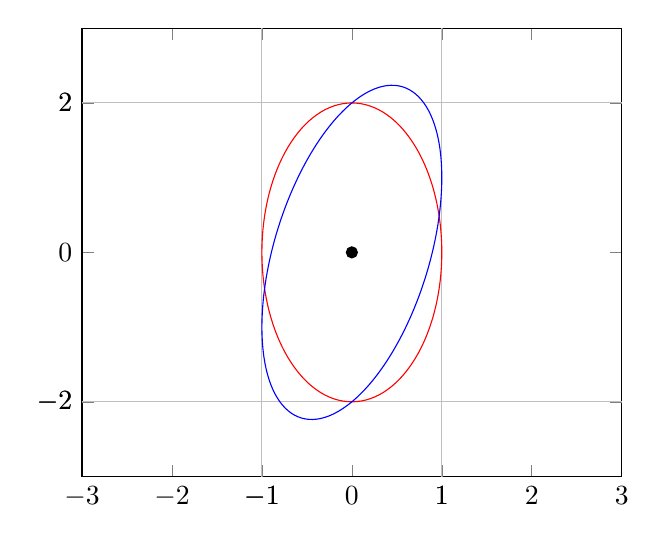
\begin{tikzpicture}
    \begin{axis}[
        xmin=-3,   xmax=3,
        ymin=-3,   ymax=3,
        extra x ticks={-1,1},
        extra y ticks={-2,2},
        extra tick style={grid=major},
    ]
        \draw[red] \pgfextra{
          \pgfpathellipse{\pgfplotspointaxisxy{0}{0}}
            {\pgfplotspointaxisdirectionxy{1}{0}}
            {\pgfplotspointaxisdirectionxy{0}{2}}
          % see also the documentation of 
          % 'axis direction cs' which
          % allows a simpler way to draw this ellipse
        };
        \draw[blue] \pgfextra{
          \pgfpathellipse{\pgfplotspointaxisxy{0}{0}}
            {\pgfplotspointaxisdirectionxy{1}{1}}
            {\pgfplotspointaxisdirectionxy{0}{2}}
        };
        \addplot [only marks,mark=*] coordinates { (0,0) };
    \end{axis}
    \end{tikzpicture}

  
  
  \begin{equation}
      x\in\mathbb{R}^{n}
  \end{equation}

  \begin{figure}[h]
    \centering
    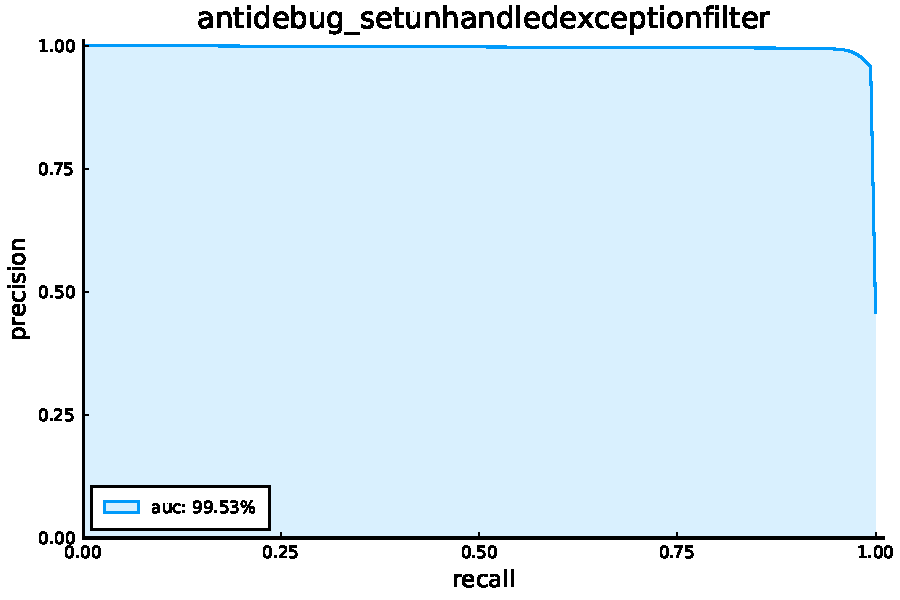
\includegraphics[width=8cm]{pdfs/modperf/antidebug_setunhandledexceptionfilter.bson-pr.pdf}
    \caption{Example of a parametric plot ($\sin (x), \cos(x), x$)}
    \label{fig:something}
  \end{figure}

  \begin{figure}
    \centering
    \begin{subfigure}{.33\textwidth}
      \centering
      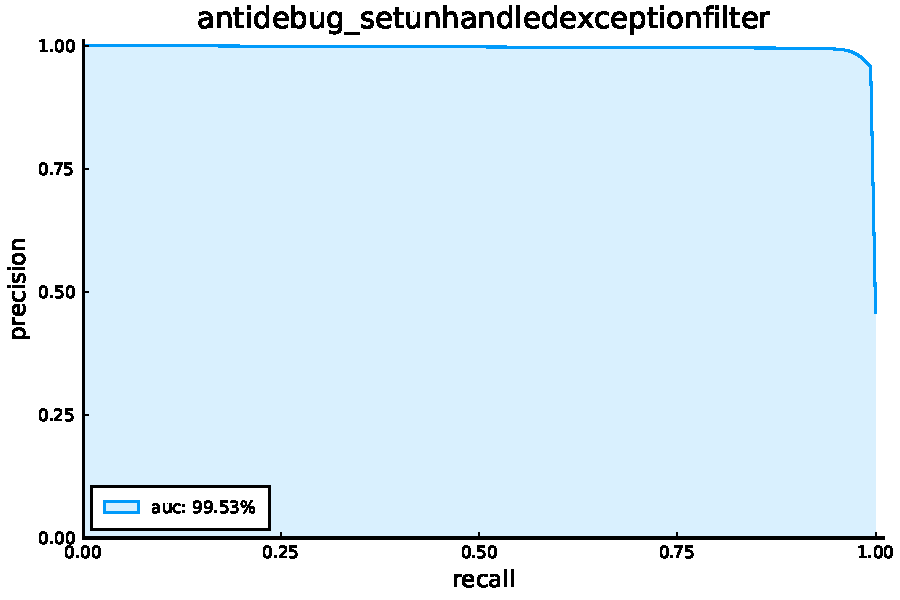
\includegraphics[width=.8\linewidth]{pdfs/modperf/antidebug_setunhandledexceptionfilter.bson-pr.pdf}
      \caption{1a}
      \label{fig:sfig1}
    \end{subfigure}%
    \begin{subfigure}{.33\textwidth}
      \centering
      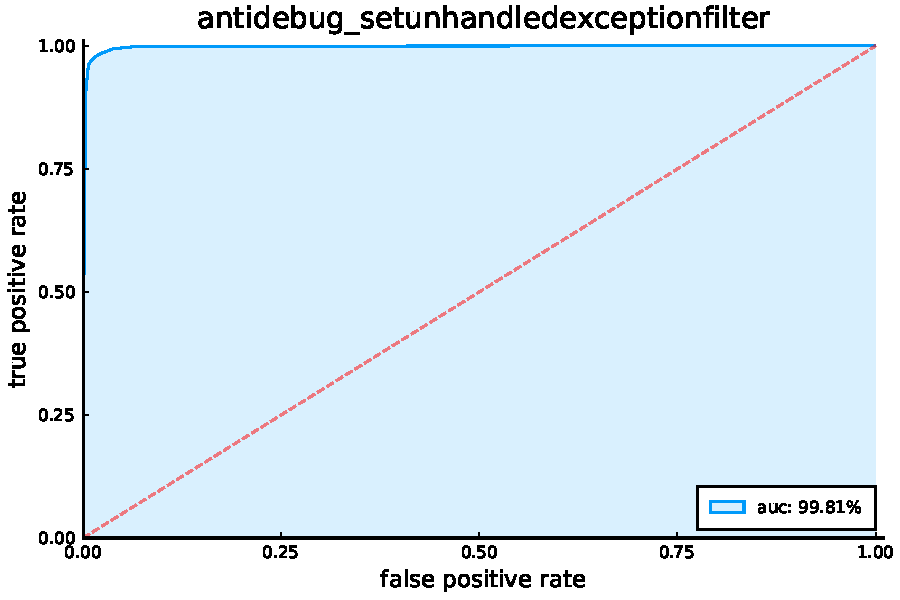
\includegraphics[width=.8\linewidth]{pdfs/modperf/antidebug_setunhandledexceptionfilter.bson-roc.pdf}
      \caption{1b}
      \label{fig:sfig2}
    \end{subfigure}
    \begin{subfigure}{.33\textwidth}
        \centering
        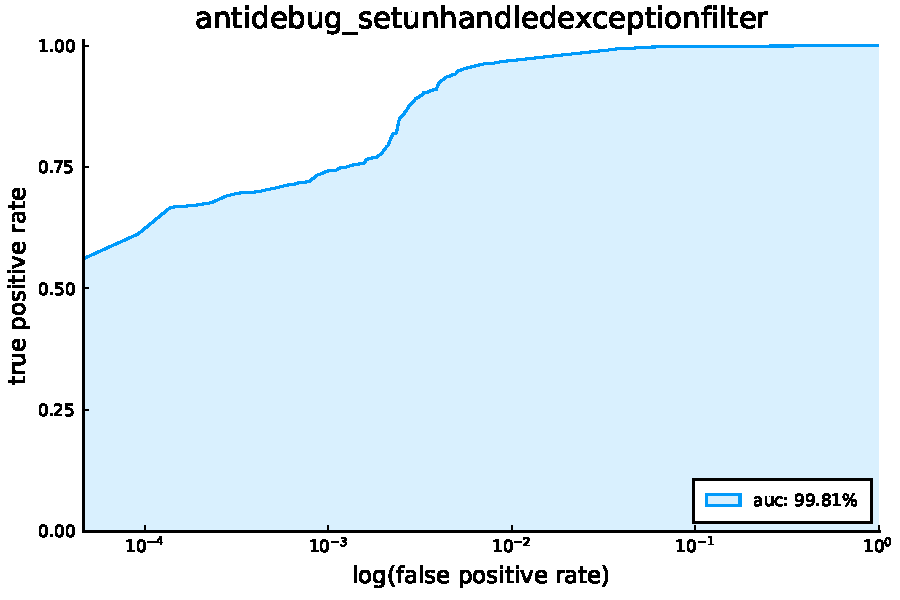
\includegraphics[width=.8\linewidth]{pdfs/modperf/antidebug_setunhandledexceptionfilter.bson-roclog.pdf}
        \caption{1c}
        \label{fig:sfig3}
    \end{subfigure}
    \caption{plots of....}
    \label{fig:fig}
\end{figure}


\begin{table}[h]
  \centering
  \caption{This is first table}
  \begin{tabular}{@{}llr@{}} \toprule
      \multicolumn{2}{c}{Item} \\ \cmidrule(r){1-2}
      Animal & Description & Price (\$)\\ \midrule
      Gnat & per gram & 13.65 \\
      & each & 0.01 \\
      Gnu & stuffed & 92.50 \\
      Emu & stuffed & 33.33 \\
      Armadillo & frozen & 8.99 \\ \bottomrule
  \end{tabular}        
\end{table}

\begin{algorithm}
  \caption{Dependency Graph Assembly}\label{algo:AKP13_command_dependency_graph_assembly}
  \begin{algorithmic}[1]
      \Procedure{MyProcedure}{}
      \State $\textit{stringlen} \gets \text{length of }\textit{string}$
      \State $i \gets \textit{patlen}$
      \If {$i > \textit{stringlen}$} \Return false
      \EndIf
      \State $j \gets \textit{patlen}$
      \If {$\textit{string}(i) = \textit{path}(j)$}
      \State $j \gets j-1$.
      \State $i \gets i-1$.
      \State \textbf{goto} \emph{loop}.
      \State \textbf{close};
      \EndIf
      \State $i \gets i+\max(\textit{delta}_1(\textit{string}(i)),\textit{delta}_2(j))$.
      \State \textbf{goto} \emph{top}.
      \EndProcedure
  \end{algorithmic}
\end{algorithm}

\tikzset{every picture/.style={line width=0.75pt}} %set default line width to 0.75pt        

\begin{center}
    \begin{tikzpicture}[x=0.75pt,y=0.75pt,yscale=-1,xscale=1]
        %uncomment if require: \path (0,269); %set diagram left start at 0, and has height of 269
        
        %Shape: Rectangle [id:dp8386354950784081] 
        \draw   (258,67) -- (301,67) -- (301,136) -- (258,136) -- cycle ;
        %Straight Lines [id:da9088407411543793] 
        \draw    (203,103) -- (257,103) ;
        \draw [shift={(259,103)}, rotate = 180] [color={rgb, 255:red, 0; green, 0; blue, 0 }  ][line width=0.75]    (10.93,-3.29) .. controls (6.95,-1.4) and (3.31,-0.3) .. (0,0) .. controls (3.31,0.3) and (6.95,1.4) .. (10.93,3.29)   ;
        %Straight Lines [id:da7684121128470209] 
        \draw    (301,103) -- (355,103) ;
        \draw [shift={(357,103)}, rotate = 180] [color={rgb, 255:red, 0; green, 0; blue, 0 }  ][line width=0.75]    (10.93,-3.29) .. controls (6.95,-1.4) and (3.31,-0.3) .. (0,0) .. controls (3.31,0.3) and (6.95,1.4) .. (10.93,3.29)   ;
        
        % Text Node
        \draw (189,94.4) node [anchor=north west][inner sep=0.75pt]    {$x$};
        % Text Node
        \draw (274,93.4) node [anchor=north west][inner sep=0.75pt]    {$f$};
        % Text Node
        \draw (362,94.4) node [anchor=north west][inner sep=0.75pt]    {$\hat{y}$};
        
        
        \end{tikzpicture}
            
\end{center}
	

	%%%%%%%%%%%%%%%%%%%%%%%%%% 
	% APPENDIX
	\appendix	

	% \printnomenclature
	% \label{apx:nomencl}
	\chapter{Used technology stack} \label{app:technologies}
\begin{enumerate}
    \item Julia
    \item Ansible
    \item Cape
\end{enumerate}


% Technology - Julia (I think I should add this in some appendix, summarize it and reference all sources used)
%   - describe why and basic features and advantages and cons
%   - Also all different codes, documented, refactored list even important libraries used in Julia
	\chapter{Model additional metrics} \label{app:models}
% Other metrics and graphs could be seen in appendix \todo{add appendix with all the data - graphs, additional metrics which are not in the body of text}

\begin{table}[h]
    \centering
    \caption{Other classifier matrix for particular signatures (rounded to 3 decimal places)}
    \begin{minipage}{\linewidth}
    \begin{tabular}{lllll}
      \toprule
      \textbf{signature} &
      \textbf{f1} &
      \textbf{AUROC} &
      \textbf{AUPRC} &
      \textbf{test loss}\footnote{logit binary cross entrophy}
      \\
      \midrule
      antidebug setunhandledexceptionfilter & 0.979 & 0.998 & 0.871 & 0.054  \\
      \midrule
      copiesself &  0.874 & 0.983 & 0.920 & 0.132 \\
      \midrule
      deletesself &  0.995 & 0.999 & 0.9997 & 0.008 \\
      \midrule
      enumerates running processes & 0.957 & 0.996 & 0.989 & 0.041 \\
      \midrule
      stealthtimeout & 0.802 & 0.794 & 0.929 &  0.263 \\
      \midrule
      useswindowsutilities & 0.945 & 0.996 & 0.987 &  0.057 \\
      \midrule
      removeszoneidads & 1.00 & 1.00 & 1.00 & 0.00 \\
      \midrule
      antisandboxsleep & 0.962 & 0.993 & 0.986 & 0.087 \\
      \midrule
      dropper & 0.840 & 0.982 & 0.902 & 0.125 \\
      \midrule
      invalid authenticode signature & 0.433 & 0.714 & 0.608 & 0.569 \\
      \midrule
      packerentropy & 0.359 & 0.776 & 0.518 & 0.436 \\
      \midrule
      stealthnetwork & 0.969 & 0.978 & 0.987 & 0.138 \\
      \bottomrule
    \end{tabular}
    \end{minipage}
    \label{tab:additional_metrics}
  \end{table}


\begin{figure}
    \centering
    \begin{subfigure}{.49\textwidth}
      \centering
      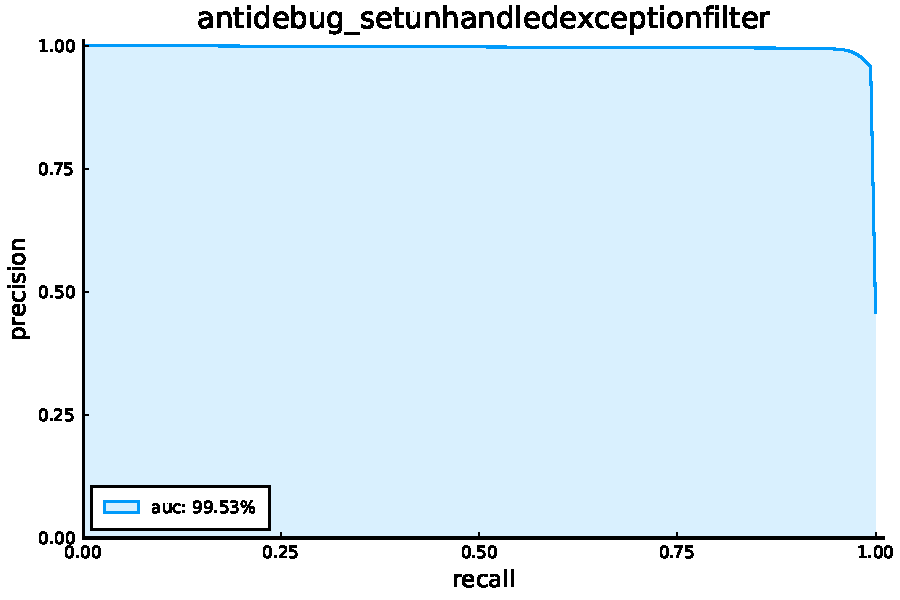
\includegraphics[width=1\linewidth]{pdfs/modperf/antidebug_setunhandledexceptionfilter.bson-pr.pdf}
      \caption{PR curve}
    \end{subfigure}
    \begin{subfigure}{.49\textwidth}
        \centering
        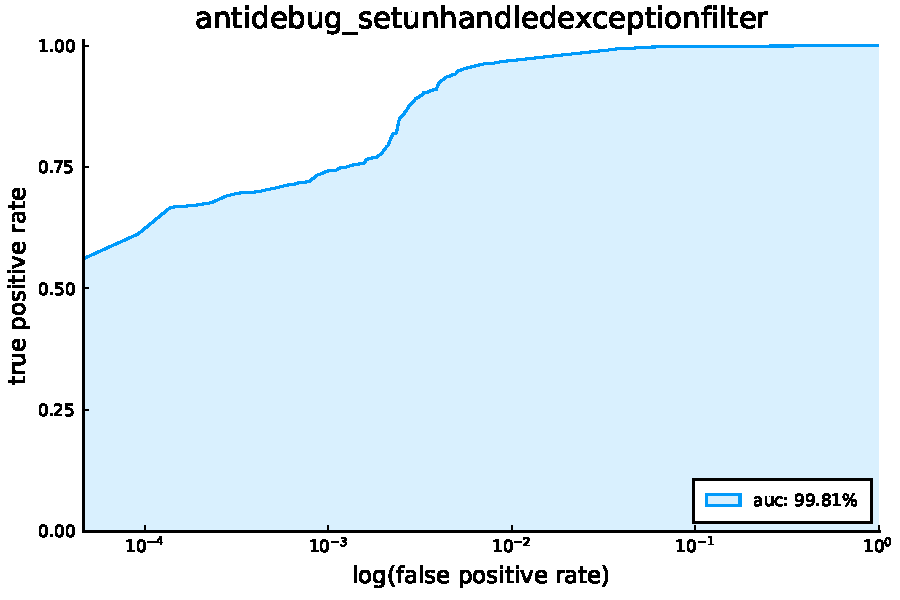
\includegraphics[width=1\linewidth]{pdfs/modperf/antidebug_setunhandledexceptionfilter.bson-roclog.pdf}
        \caption{ROC (log on x-axis)}
        % \label{fig:sfig3}
    \end{subfigure}
    \caption{antidebug setunhandledexceptionfilter plots}
    \label{fig:fig}
\end{figure}

\begin{figure}
    \centering
    \begin{subfigure}{.49\textwidth}
      \centering
      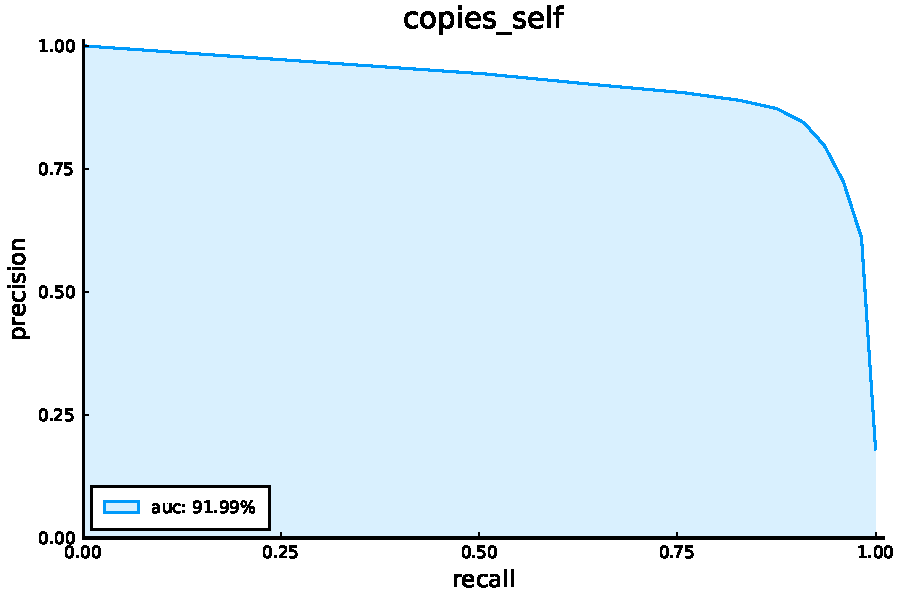
\includegraphics[width=1\linewidth]{pdfs/modperf/copies_self.bson-pr.pdf}
      \caption{PR curve}
    \end{subfigure}
    \begin{subfigure}{.49\textwidth}
        \centering
        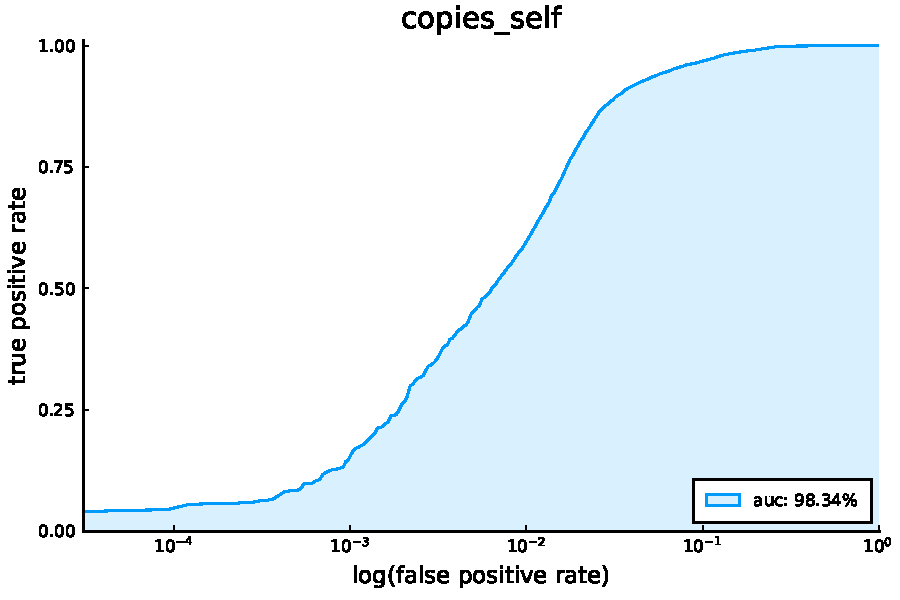
\includegraphics[width=1\linewidth]{pdfs/modperf/copies_self.bson-roclog.pdf}
        \caption{ROC (log on x-axis)}
        % \label{fig:sfig3}
    \end{subfigure}
    \caption{copiesself plots}
    \label{fig:fig}
\end{figure}

\begin{figure}
    \centering
    \begin{subfigure}{.49\textwidth}
      \centering
      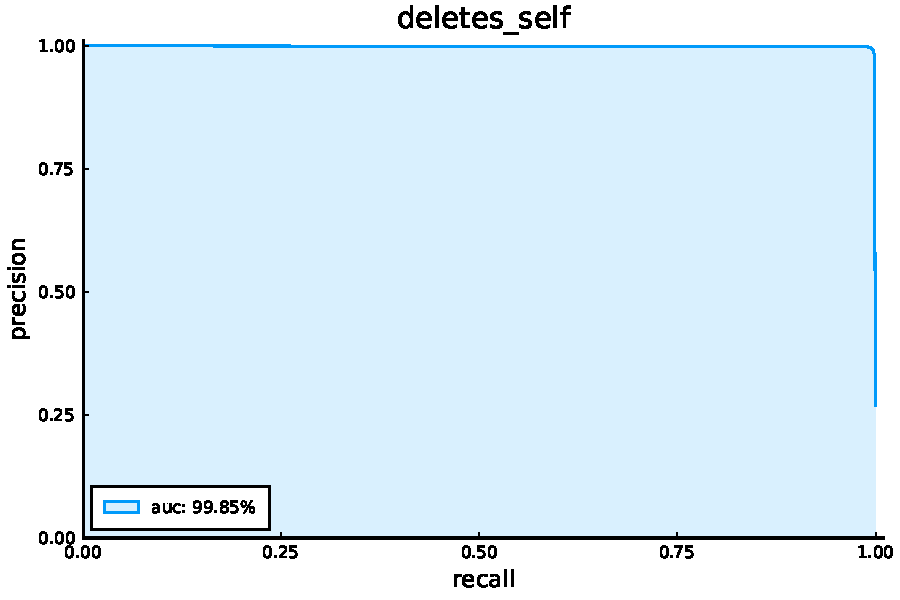
\includegraphics[width=1\linewidth]{pdfs/modperf/deletes_self.bson-pr.pdf}
      \caption{PR curve}
    \end{subfigure}
    \begin{subfigure}{.49\textwidth}
        \centering
        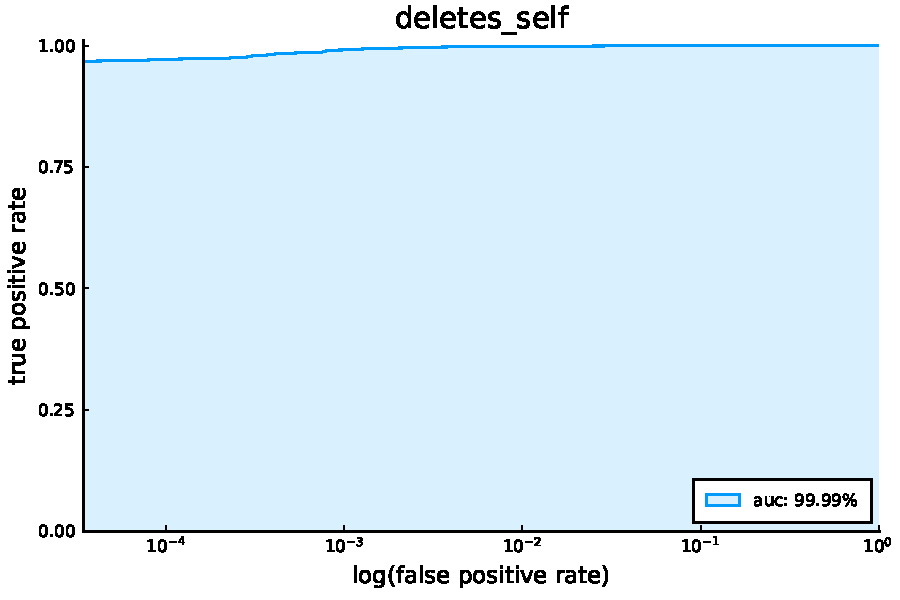
\includegraphics[width=1\linewidth]{pdfs/modperf/deletes_self.bson-roclog.pdf}
        \caption{ROC (log on x-axis)}
        % \label{fig:sfig3}
    \end{subfigure}
    \caption{deletesself plots}
    \label{fig:fig}
\end{figure}

\begin{figure}
    \centering
    \begin{subfigure}{.49\textwidth}
      \centering
      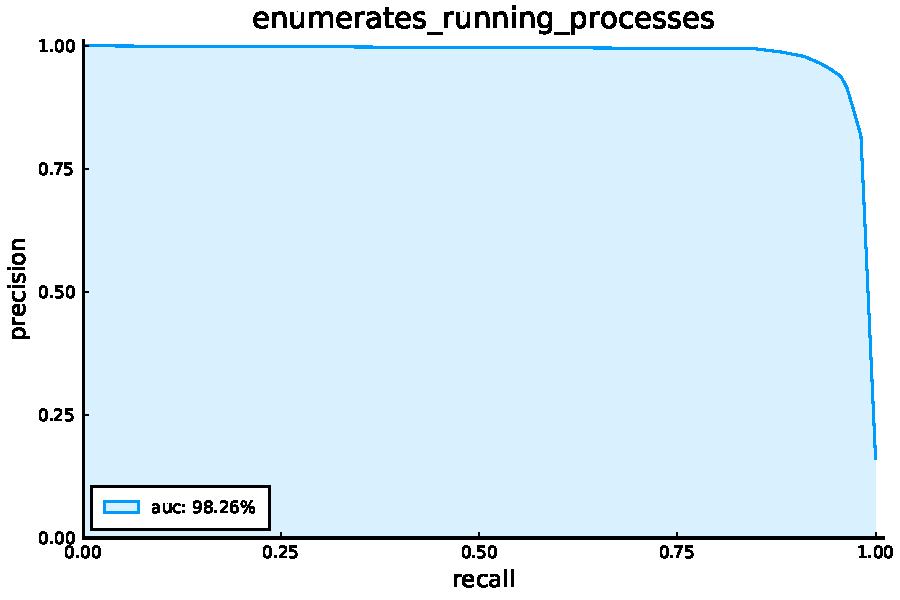
\includegraphics[width=1\linewidth]{pdfs/modperf/enumerates_running_processes.bson-pr.pdf}
      \caption{PR curve}
    \end{subfigure}
    \begin{subfigure}{.49\textwidth}
        \centering
        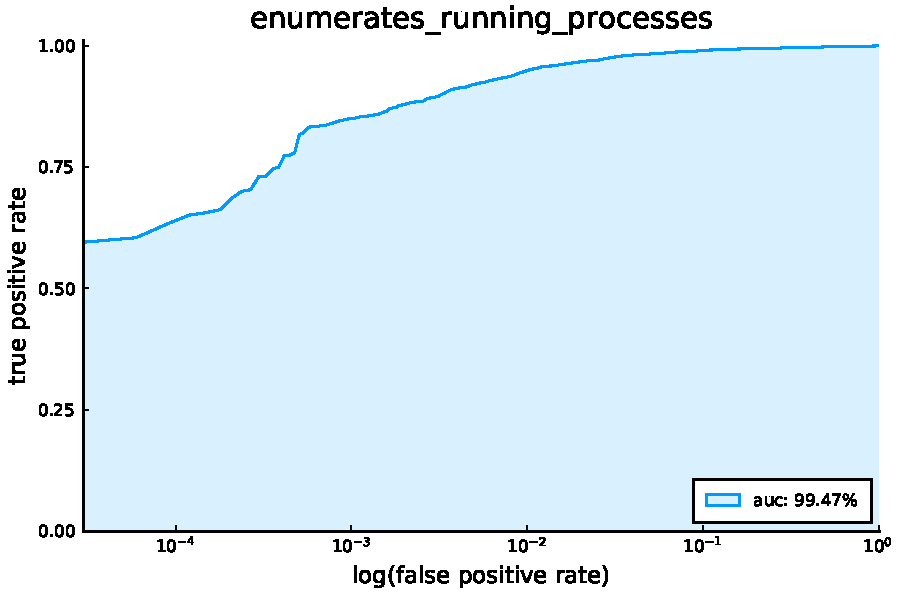
\includegraphics[width=1\linewidth]{pdfs/modperf/enumerates_running_processes.bson-roclog.pdf}
        \caption{ROC (log on x-axis)}
        % \label{fig:sfig3}
    \end{subfigure}
    \caption{enumerates running processes plots}
    \label{fig:fig}
\end{figure}

\begin{figure}
    \centering
    \begin{subfigure}{.49\textwidth}
      \centering
      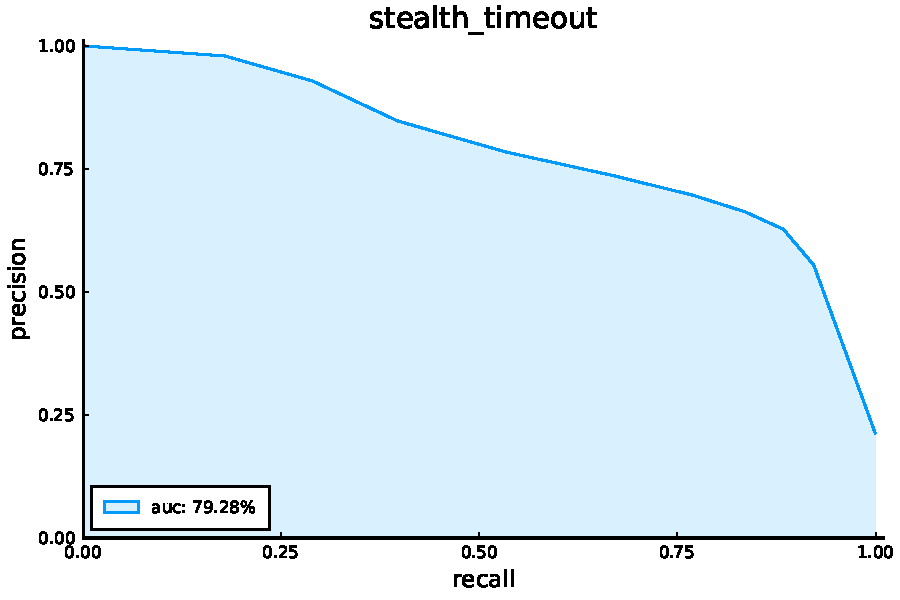
\includegraphics[width=1\linewidth]{pdfs/modperf/stealth_timeout.bson-pr.pdf}
      \caption{PR curve}
    \end{subfigure}
    \begin{subfigure}{.49\textwidth}
        \centering
        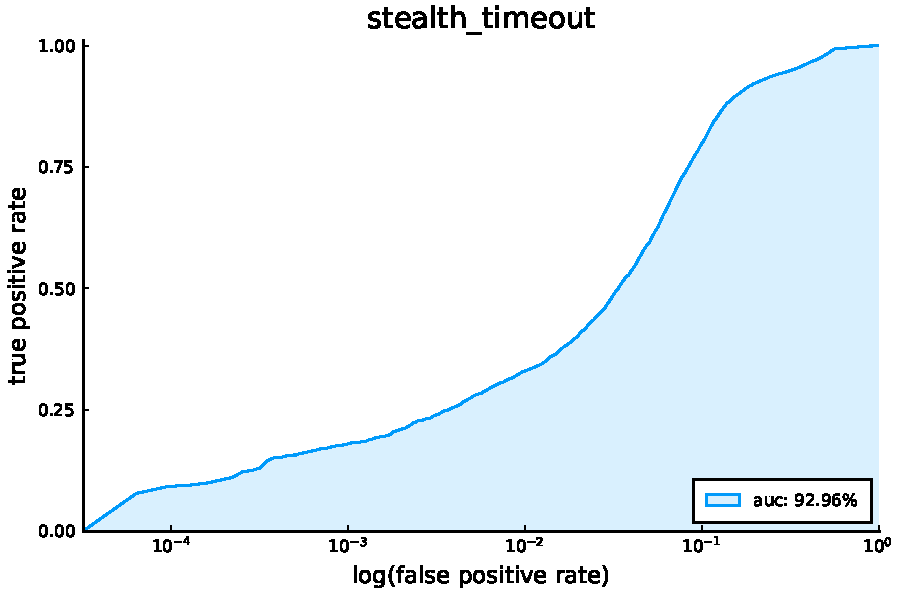
\includegraphics[width=1\linewidth]{pdfs/modperf/stealth_timeout.bson-roclog.pdf}
        \caption{ROC (log on x-axis)}
        % \label{fig:sfig3}
    \end{subfigure}
    \caption{stealthtimeout plots}
    \label{fig:fig}
\end{figure}

\begin{figure}
    \centering
    \begin{subfigure}{.49\textwidth}
      \centering
      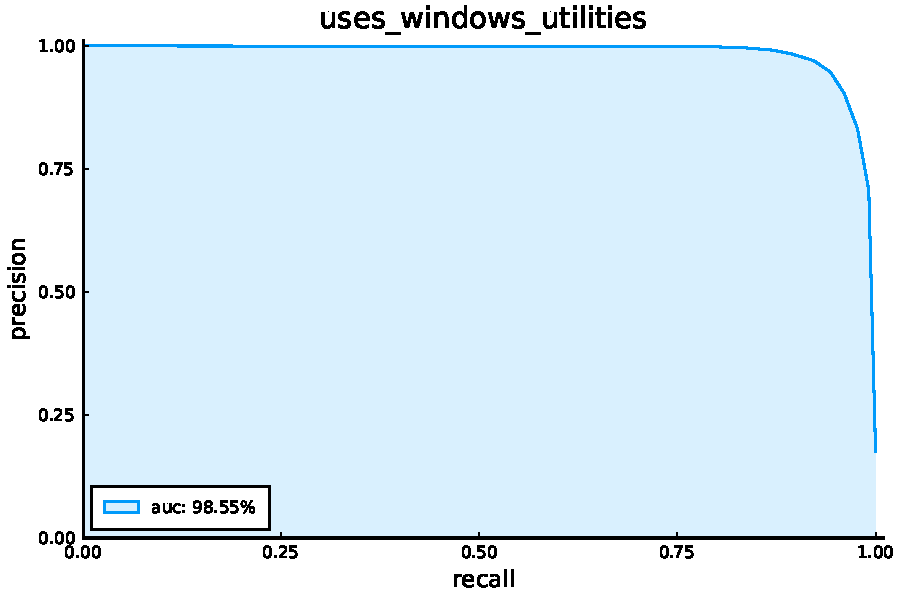
\includegraphics[width=1\linewidth]{pdfs/modperf/uses_windows_utilities.bson-pr.pdf}
      \caption{PR curve}
    \end{subfigure}
    \begin{subfigure}{.49\textwidth}
        \centering
        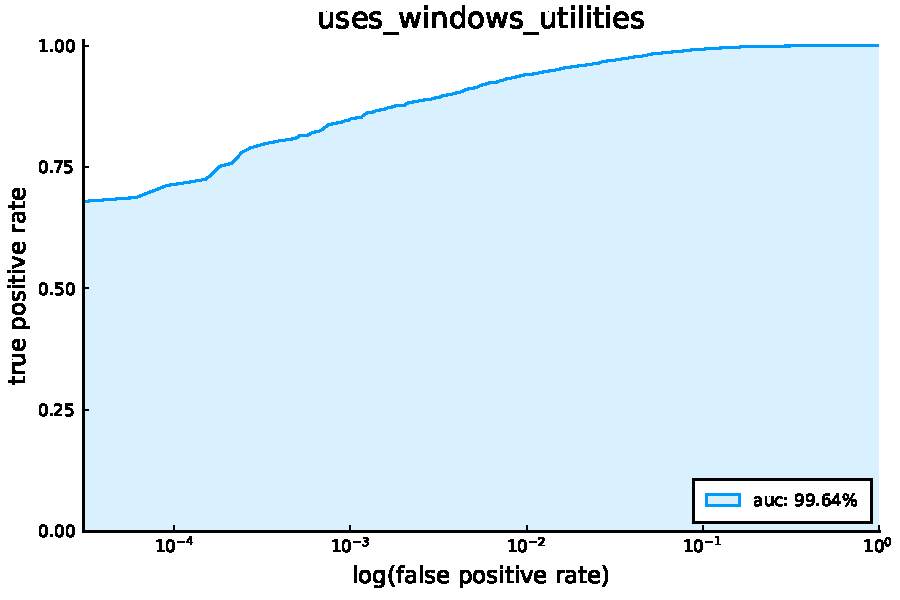
\includegraphics[width=1\linewidth]{pdfs/modperf/uses_windows_utilities.bson-roclog.pdf}
        \caption{ROC (log on x-axis)}
        % \label{fig:sfig3}
    \end{subfigure}
    \caption{uses windows utilities plots}
    \label{fig:fig}
\end{figure}

\begin{figure}
    \centering
    \begin{subfigure}{.49\textwidth}
      \centering
      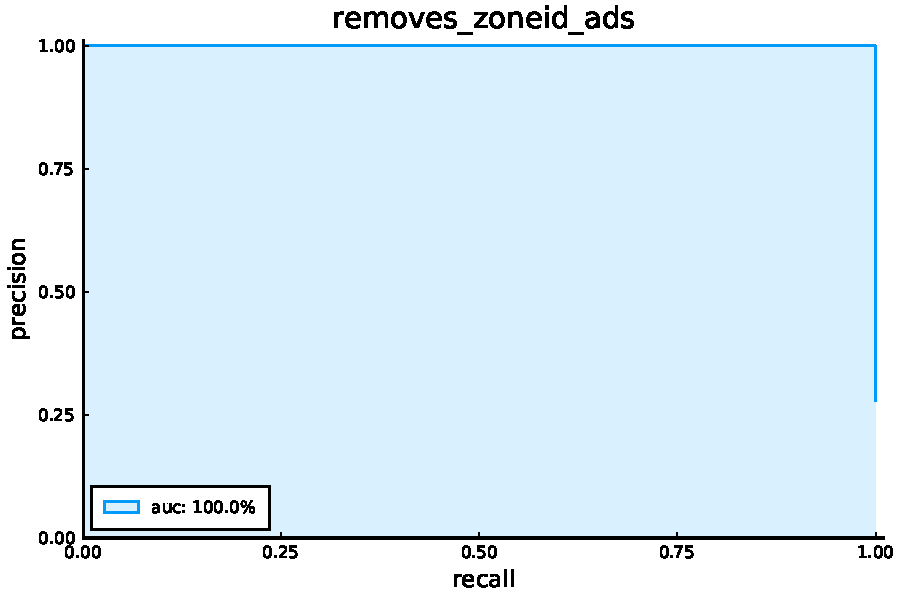
\includegraphics[width=1\linewidth]{pdfs/modperf/removes_zoneid_ads.bson-pr.pdf}
      \caption{PR curve}
    \end{subfigure}
    \begin{subfigure}{.49\textwidth}
        \centering
        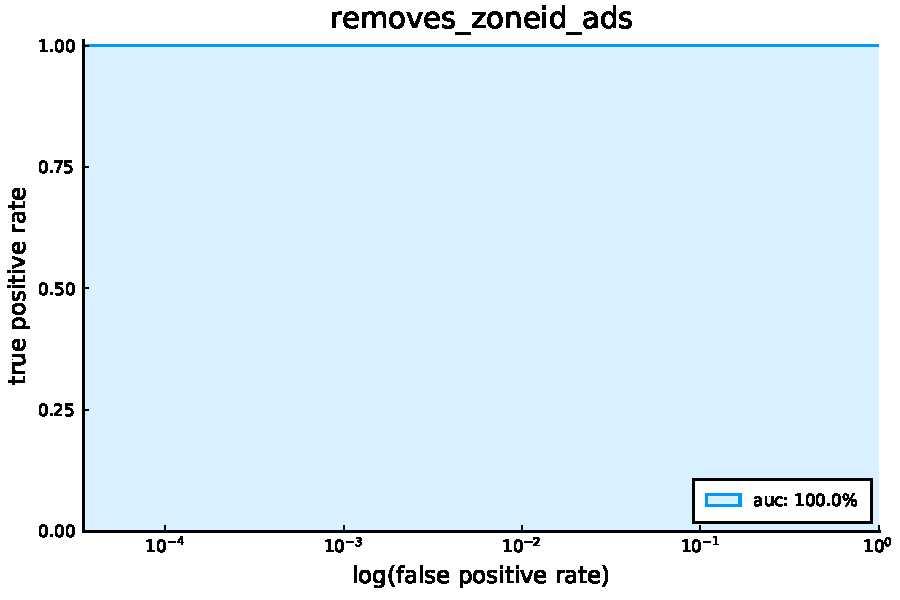
\includegraphics[width=1\linewidth]{pdfs/modperf/removes_zoneid_ads.bson-roclog.pdf}
        \caption{ROC (log on x-axis)}
        % \label{fig:sfig3}
    \end{subfigure}
    \caption{removeszoneidads plots}
    \label{fig:fig}
\end{figure}

\begin{figure}
    \centering
    \begin{subfigure}{.49\textwidth}
      \centering
      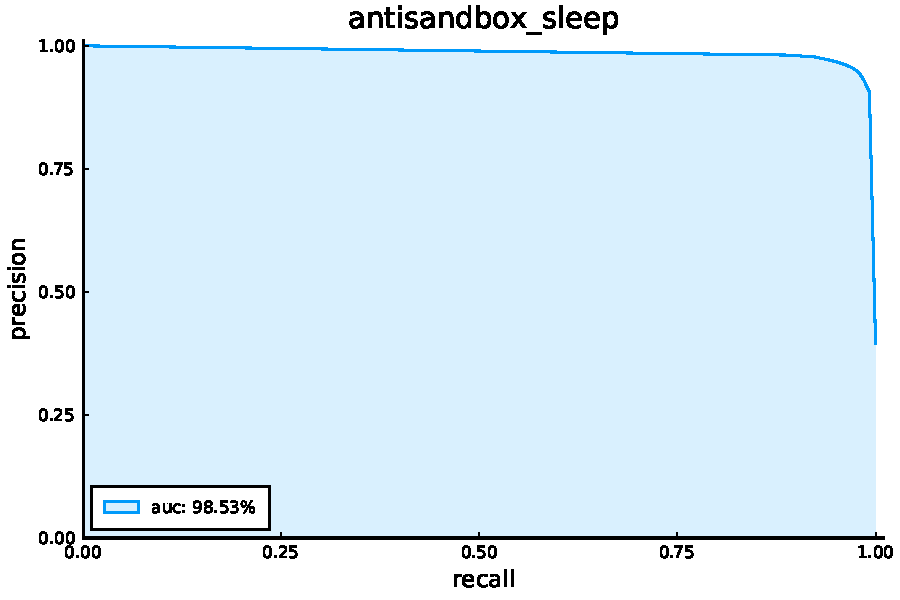
\includegraphics[width=1\linewidth]{pdfs/modperf/antisandbox_sleep.bson-pr.pdf}
      \caption{PR curve}
    \end{subfigure}
    \begin{subfigure}{.49\textwidth}
        \centering
        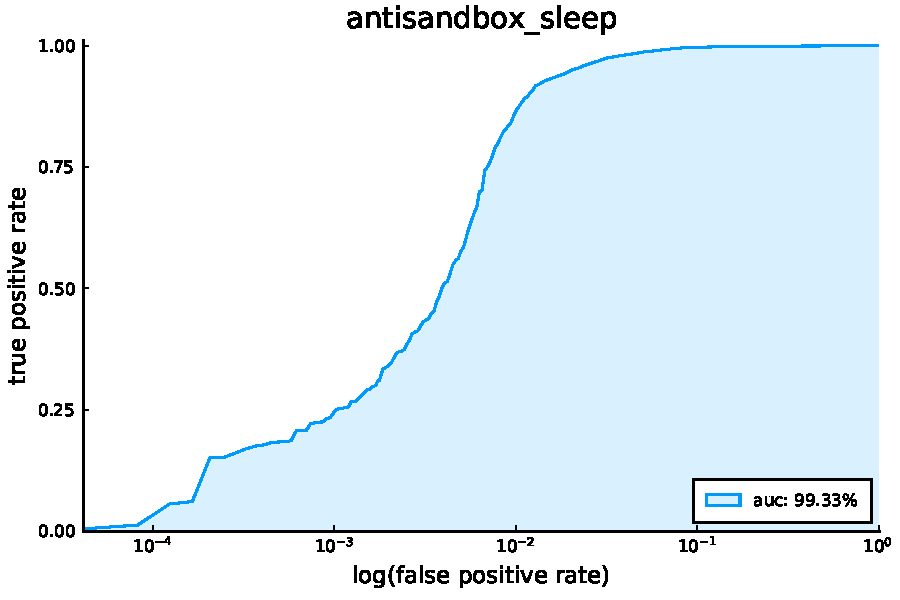
\includegraphics[width=1\linewidth]{pdfs/modperf/antisandbox_sleep.bson-roclog.pdf}
        \caption{ROC (log on x-axis)}
        % \label{fig:sfig3}
    \end{subfigure}
    \caption{antisandboxsleep plots}
    \label{fig:fig}
\end{figure}

\begin{figure}
    \centering
    \begin{subfigure}{.49\textwidth}
      \centering
      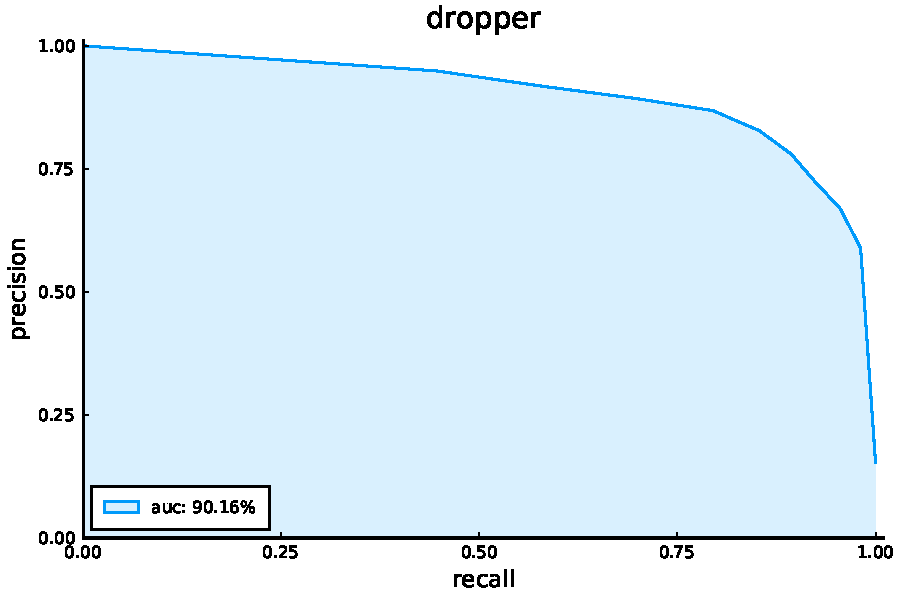
\includegraphics[width=1\linewidth]{pdfs/modperf/dropper.bson-pr.pdf}
      \caption{PR curve}
    \end{subfigure}
    \begin{subfigure}{.49\textwidth}
        \centering
        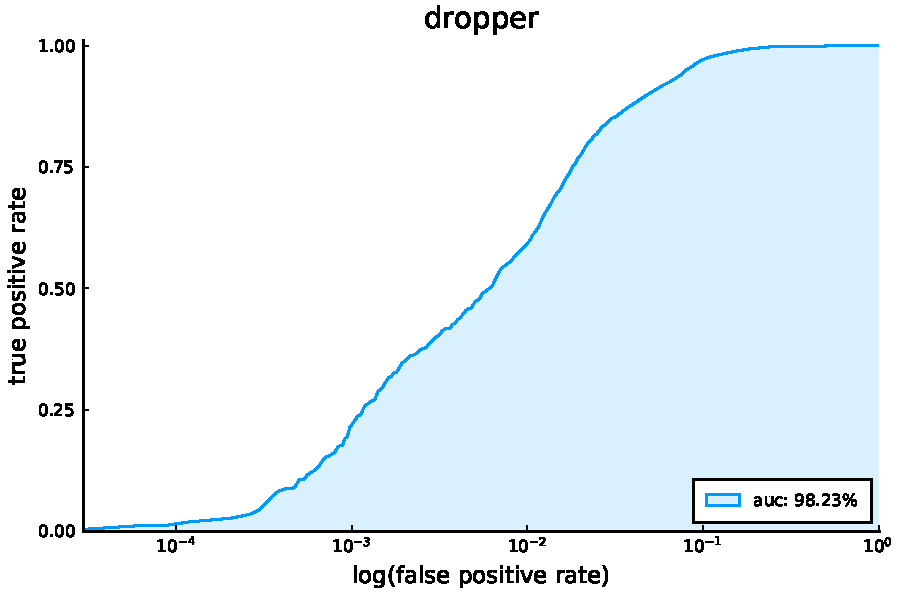
\includegraphics[width=1\linewidth]{pdfs/modperf/dropper.bson-roclog.pdf}
        \caption{ROC (log on x-axis)}
        % \label{fig:sfig3}
    \end{subfigure}
    \caption{antidebug dropper plots}
    \label{fig:fig}
\end{figure}

\begin{figure}
    \centering
    \begin{subfigure}{.49\textwidth}
      \centering
      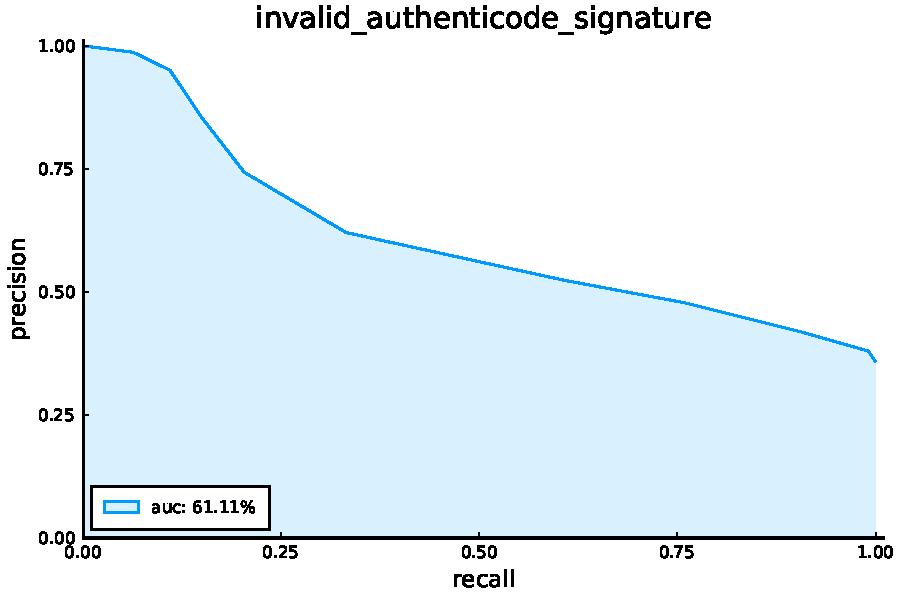
\includegraphics[width=1\linewidth]{pdfs/modperf/invalid_authenticode_signature.bson-pr.pdf}
      \caption{PR curve}
    \end{subfigure}
    \begin{subfigure}{.49\textwidth}
        \centering
        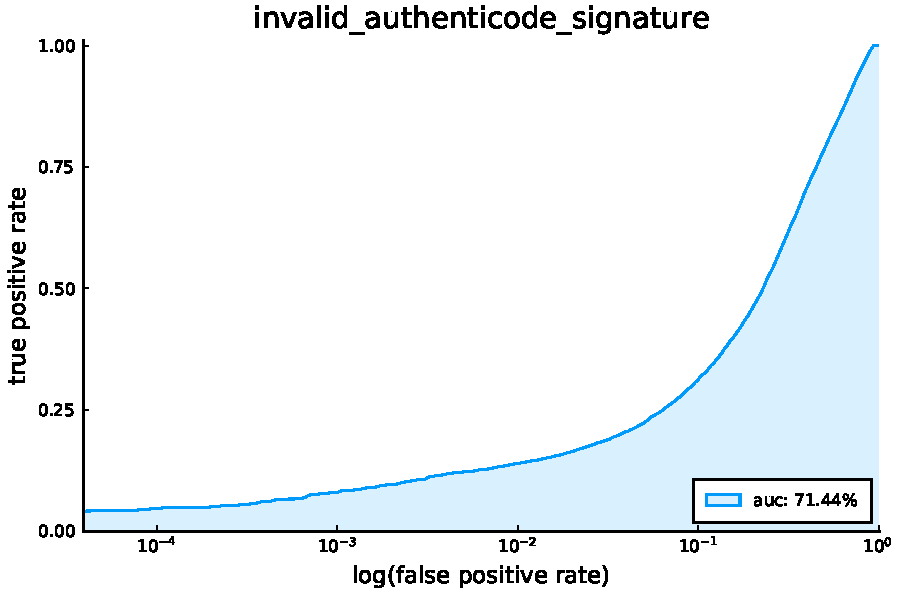
\includegraphics[width=1\linewidth]{pdfs/modperf/invalid_authenticode_signature.bson-roclog.pdf}
        \caption{ROC (log on x-axis)}
        % \label{fig:sfig3}
    \end{subfigure}
    \caption{invalid authenticode signature plots}
    \label{fig:fig}
\end{figure}

\begin{figure}
    \centering
    \begin{subfigure}{.49\textwidth}
      \centering
      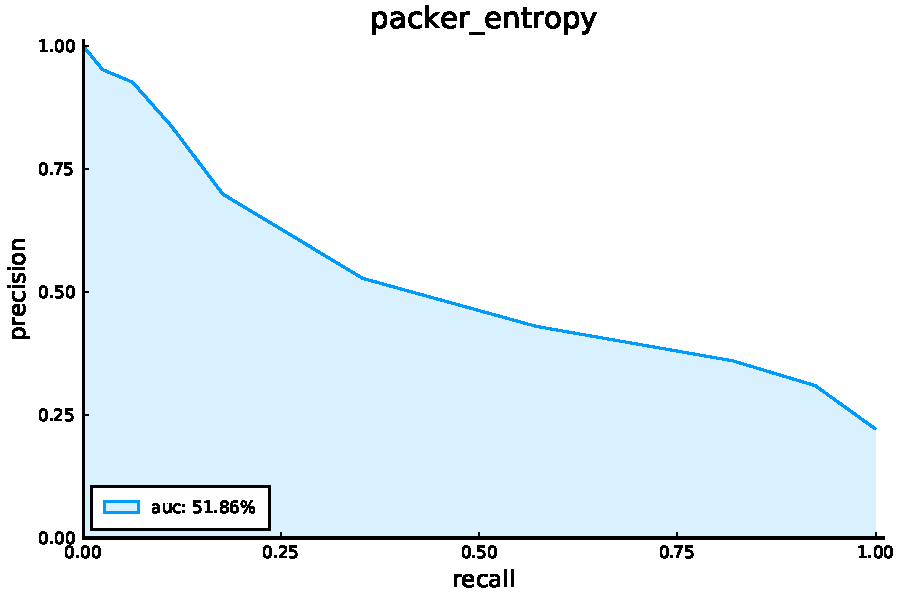
\includegraphics[width=1\linewidth]{pdfs/modperf/packer_entropy.bson-pr.pdf}
      \caption{PR curve}
    \end{subfigure}
    \begin{subfigure}{.49\textwidth}
        \centering
        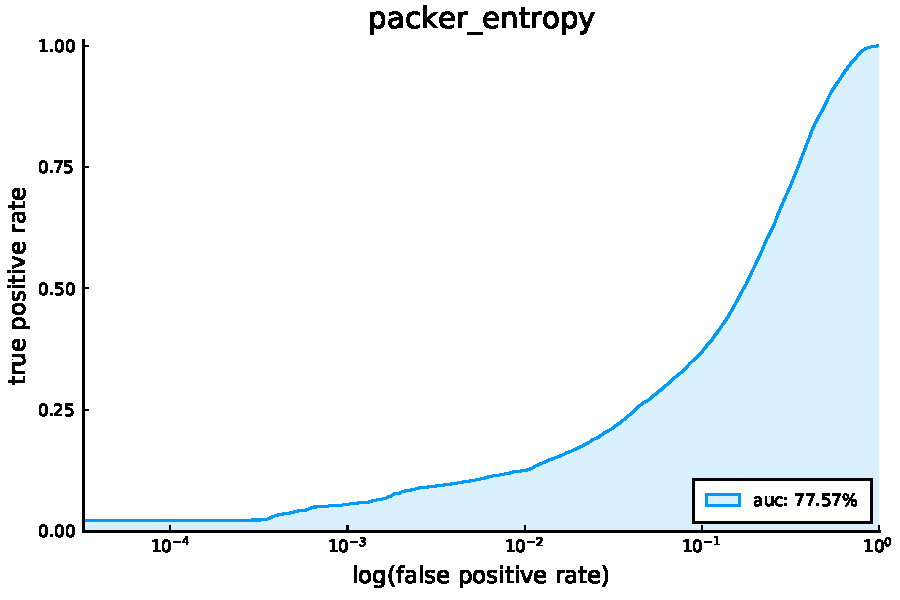
\includegraphics[width=1\linewidth]{pdfs/modperf/packer_entropy.bson-roclog.pdf}
        \caption{ROC (log on x-axis)}
        % \label{fig:sfig3}
    \end{subfigure}
    \caption{packerentropy plots}
    \label{fig:fig}
\end{figure}

\begin{figure}
    \centering
    \begin{subfigure}{.49\textwidth}
      \centering
      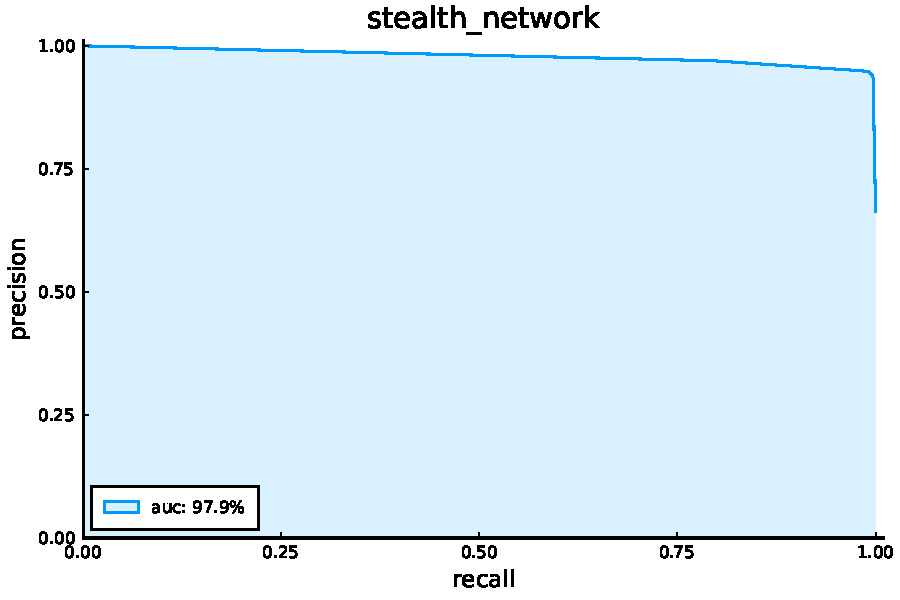
\includegraphics[width=1\linewidth]{pdfs/modperf/stealth_network.bson-pr.pdf}
      \caption{PR curve}
    \end{subfigure}
    \begin{subfigure}{.49\textwidth}
        \centering
        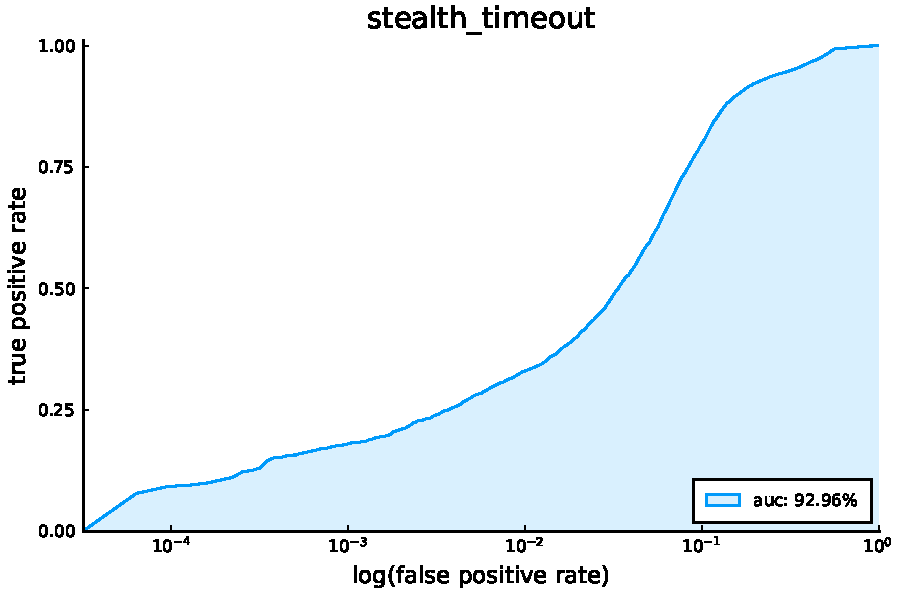
\includegraphics[width=1\linewidth]{pdfs/modperf/stealth_timeout.bson-roclog.pdf}
        \caption{ROC (log on x-axis)}
        % \label{fig:sfig3}
    \end{subfigure}
    \caption{stealthnetwork plots}
    \label{fig:fig}
\end{figure}





% f-score, auroc,auprc, loss
% PR curve, ROC curve log

	\printglossary[type=\acronymtype]

	%Biblio
	\bibliographystyle{alpha}
	%\bibliographystyle{csplainnat}
	%bibliographystyle{plain}
	% \bibliographystyle{psc}
	%\bibliographystyle{apalike}
	{
	\bibliography{bib/Master_thesis}
	}

	% \chapter{Obsah přiloženého CD}
	% \textbf{\large Tato příloha je povinná pro každou práci. Každá práce musí totiž obsahovat přiložené CD. Viz dále.}

	% Může vypadat například takto. Váš seznam samozřejmě bude odpovídat typu vaší práce. (viz \cite{infodp}):

	% \begin{figure}[h]
	% \begin{center}
	% \includegraphics[width=14cm]{figures/seznamcd}
	% \caption{Seznam přiloženého CD --- příklad}
	% \label{fig:seznamcd}
	% \end{center}
	% \end{figure}

	% Na GNU/Linuxu si strukturu přiloženého CD můžete snadno vyrobit příkazem:\\ 
	% \verb|$ tree . >tree.txt|\\
	% Ve vzniklém souboru pak stačí pouze doplnit komentáře.

	% Z \textbf{README.TXT} (případne index.html apod.)  musí být rovněž zřejmé, jak programy instalovat, spouštět a jaké požadavky mají tyto programy na hardware.

	% Adresář \textbf{text}  musí obsahovat soubor s vlastním textem práce v PDF nebo PS formátu, který bude později použit pro prezentaci diplomové práce na WWW.

\end{document}
